% LaTeX version of thesis_quarto_manuscript.qmd
%
% Tables, figures and in-text numbers are read from output/, which is generated by the R scripts
% in code/ (run code/run_all.R from the project root). To compile on Overleaf, upload this file
% together with bibliography.bib, output/ and survey_screenshots/.
%
% Compiles with XeLaTeX (closest match to the quarto PDF; set Menu > Compiler > XeLaTeX on Overleaf),
% LuaLaTeX or pdfLaTeX. The bibliography is built with biber, which Overleaf runs automatically.

\PassOptionsToPackage{unicode}{hyperref}
\PassOptionsToPackage{hyphens}{url}
\PassOptionsToPackage{dvipsnames,svgnames,x11names}{xcolor}

% The quarto YAML's fontsize "12" is not a valid class option, so the quarto PDF was set at 11pt
\documentclass[11pt, letterpaper, DIV=11, numbers=noendperiod]{scrartcl}

%---------------------------------------------------------------------------------------------------
% Fonts: Times body text and maths with Garamond headings, as in the quarto PDF
% (Times New Roman, Garamond and Cambria Math are not available on Overleaf, so free equivalents are used)
%---------------------------------------------------------------------------------------------------

\usepackage{amsmath}
\usepackage{iftex}
\ifPDFTeX
  \usepackage[T1]{fontenc}
  \usepackage[utf8]{inputenc}
  \usepackage{newtxtext}
  \usepackage{newtxmath}
  \renewcommand*{\sfdefault}{EBGaramond-LF}
\else
  \usepackage{unicode-math}
  \defaultfontfeatures{Scale=MatchLowercase}
  \defaultfontfeatures[\rmfamily]{Ligatures=TeX,Scale=1}
  \setmainfont{texgyretermes}[Extension=.otf, UprightFont=*-regular, BoldFont=*-bold,
    ItalicFont=*-italic, BoldItalicFont=*-bolditalic]
  \setsansfont{EBGaramond}[Extension=.otf, UprightFont=*-Regular, BoldFont=*-Bold,
    ItalicFont=*-Italic, BoldItalicFont=*-BoldItalic]
  \setmathfont{texgyretermes-math.otf}
\fi
\usepackage{microtype}

%---------------------------------------------------------------------------------------------------
% Page layout: double spacing, indented paragraphs, unnumbered sections with centred section titles
%---------------------------------------------------------------------------------------------------

\usepackage{setspace}
\KOMAoptions{parskip=half}
\usepackage{indentfirst}
\setlength{\parindent}{3em}
\setlength{\emergencystretch}{3em}
\setcounter{secnumdepth}{-\maxdimen}

\usepackage{etoolbox}
\makeatletter
\renewcommand*{\sectionlinesformat}[4]{% centre section titles; subsection titles stay left-aligned
  \ifstrequal{#1}{section}{\centering #3#4}{\@hangfrom{\hskip #2#3}{#4}}}
\makeatother

\usepackage{enumitem}
\setlist[itemize]{topsep=0pt,itemsep=0pt,partopsep=0pt,parsep=0pt}
\setlist[enumerate]{topsep=0pt,itemsep=0pt,partopsep=0pt,parsep=0pt}
\providecommand{\tightlist}{\setlength{\itemsep}{0pt}\setlength{\parskip}{0pt}}

%---------------------------------------------------------------------------------------------------
% Tables and figures: packages used by the gt (gtsummary) and texreg tables in output/tables,
% with captions below tables as in the quarto PDF
%---------------------------------------------------------------------------------------------------

\usepackage{graphicx}
\usepackage{float}
\usepackage{booktabs}
\usepackage{longtable}
\usepackage{array}
\usepackage{calc}
\usepackage{colortbl}
\usepackage{multirow}
\usepackage{anyfontsize}
\usepackage{caption}
\usepackage{subcaption}
\KOMAoption{captions}{tablesignature}
\makeatletter
\def\fps@figure{htbp}
\makeatother

%---------------------------------------------------------------------------------------------------
% Bibliography: Chicago author-date, as rendered by quarto's default citation style
%---------------------------------------------------------------------------------------------------

\usepackage[english]{babel}
\usepackage{csquotes}
\usepackage[authordate, backend=biber, compresspages, footmarkoff]{biblatex-chicago} % footmarkoff keeps KOMA's footnote style
\addbibresource{bibliography.bib}

% Print the same fields as quarto's citation style: no ISSN/ISBN, access dates, months or languages
\AtEveryBibitem{%
  \clearfield{issn}\clearfield{isbn}\clearfield{month}\clearlist{language}%
  \clearfield{urlyear}\clearfield{urlmonth}\clearfield{urlday}}

% Show the status of unpublished papers, which Zotero exports in the type field
\DeclareSourcemap{\maps[datatype=bibtex]{\map{\pertype{unpublished}\step[fieldsource=type, fieldtarget=note]}}}

%---------------------------------------------------------------------------------------------------
% Links and PDF metadata
%---------------------------------------------------------------------------------------------------

\usepackage{xcolor}
\usepackage{xurl}
\usepackage{bookmark}
\urlstyle{same}
\hypersetup{
  pdftitle={Too hard to get: the role of probabilistic expectations and cognitive complexity in multi-dimensional reference dependence},
  pdfauthor={Aspen Han},
  colorlinks=true,
  linkcolor={blue},
  filecolor={Maroon},
  citecolor={black}, % citations are linked to the bibliography but, as in the quarto PDF, not coloured
  urlcolor={Blue}}

%---------------------------------------------------------------------------------------------------
% Numbers cited in the text, generated by code/descriptive_tables.R and code/regression_test.R
%---------------------------------------------------------------------------------------------------

% Generated by the R scripts in code/; do not edit by hand
\newcommand{\NumObs}{642}
\newcommand{\NumObsLab}{213}
\newcommand{\NumObsClass}{429}
\newcommand{\NumObsMicro}{233}
\newcommand{\NumObsMacro}{196}
\newcommand{\NumRespondents}{797}
\newcommand{\BalanceLabChisq}{82.33}
\newcommand{\BalanceLabPval}{0.13}

% Generated by the R scripts in code/; do not edit by hand
\newcommand{\ControlMeanSets}{23.61}


\title{Too hard to get: the role of probabilistic expectations and cognitive complexity in multi-dimensional reference dependence}
\author{Aspen Han}
\date{}

\begin{document}

\maketitle

\setstretch{2}

\newpage

\section{Abstract}\label{abstract}

This paper seeks to investigate the effects of conflicting reference points across different dimensions of utility on effort exertion. Reference-dependent preference models so far have assumed additive separability across different dimensions of utility, which implies that agents respond to reference points in each dimension in isolation from one another. Challenging this assumption, this paper posits that agents consider multi-dimensional reference points in tandem: agents are less responsive to reference points if they have low probabilistic expectations of being able to concurrently achieve them and/or if they have difficulty reconciling them into a single baseline against which to evaluate outcomes. It refines the Koszegi-Rabin reference-dependent preference model to incorporate these effects and applies it to examine effort exertion under targets in different task performance dimensions. The original and refined model produce distinct predictions for optimal effort exertion, which are tested via a real effort experiment. However, the experimental results are inconclusive, finding some evidence of attenuation but which is not statistically significant nor robust. They do shed light on dynamics between internally conceived and externally imposed targets and how they enter into reference point formation which has bearing for target design and can be a promising new area of research for the future.

\newpage

\section{Acknowledgements}\label{acknowledgements}

Special thanks to

\begin{itemize}
\tightlist
\item
  Professor Fulya Ersoy for advising this thesis, including refining the research idea and experimental design, obtaining IRB approval, and providing feedback on my writing
\item
  Professors Min Sok Lee and Kanit (Ken) Kuevibulvanich for helping to run the experiment with their classes
\item
  The RF-CDR team for helping to run the experiment at their lab, namely

  \begin{itemize}
  \tightlist
  \item
    Nina Semushina
  \item
    Lucia Agajanian
  \item
    Justin Daugherty
  \item
    Akshaj Dwivedula
  \item
    Pablo Paucar
  \item
    Angelysse Madsen
  \item
    Adam Vargas
  \item
    Kaushal Addanki
  \item
    Charlotte Parque
  \end{itemize}
\item
  My friends Elliot Lin, Lim Mian, Nour Abdelbaki and others who helped to test and debug the survey and provided moral support
\end{itemize}

\newpage

\section{Introduction}\label{introduction}

Consider the employee of a firm whose performance is evaluated against targets across various performance dimensions (e.g.~production speed, accuracy, quality etc). For example, an assembly line worker in an electronics manufacturing plant could be subject to targets on the number of components made per hour (speed), the proportion of defective components made (accuracy), and the average durability of components made (quality). Similarly in the service sector, an Uber driver could be evaluated on the number of rides provided per month, average mileage per unit time, and the average customer satisfaction rating. It is apparent that tensions between these performance dimensions can surface, which can affect the targets' effectiveness as motivators. The emphasis for consistency and complementarity between different performance dimensions, including targets set in each, is strongly echoed in operations and general management literature \parencite[e.g.][]{hayes.1984.restoringour,hayes.1978.howshould,skinner.1974.focusedfactory,skinner.1996.manufacturingstrategy,swamidass.2000.focusedfactory}. Further insights can be gleaned from examining this concept within economics. Targets can and have been integrated into the framework of expectations-based reference points \parencite{heath.1999.goalsreference,vonrechenberg.2016.goalsreference}, a growing body of research within behavioral economics. However, empirical studies have mainly examined the effects of reference points uni-dimensionally, though theoretical models encompassing multi-dimensional reference points exist. Thus, I seek to investigate the mechanisms through which reference points interact across dimensions within this economic framework, specifically answering the following research questions:

\begin{enumerate}
\def\labelenumi{\arabic{enumi}.}
\tightlist
\item
  Do probabilistic beliefs about the achievability of reference points across multiple dimensions affect how responsive agents are to said reference points?
\item
  Does cognitive complexity in reconciling reference points across multiple dimensions affect how responsive agents are to said reference points?
\end{enumerate}

This research is theoretically founded on the \textcite{koszegi.2006.modelreferencedependenta} model of reference-dependence (henceforth KR model), which builds upon Kahneman and Tversky's \parencite*{kahneman.1979.prospecttheory,tversky.1991.lossaversion} prospect theory and related models of regret and disappointment \parencite[e.g.][]{bell.1982.regretdecision,bell.1985.disappointmentdecision,loomes.1982.regrettheory,loomes.1986.disappointmentdynamic,gul.1991.theorydisappointment}. Defining features of this overarching framework include the evaluation of outcomes relative to a reference point rather than on absolute terms, weighting losses more than gains, diminishing sensitivity away from the reference point, and decision weights on outcomes which are transformations of objective probabilities. A major contribution by the KR model is that it constructs a source for the reference points to be the agent's (rational) expectations, specifically his/her probabilistic beliefs held in the recent past about what will or should happen. This accommodated alternative arguments about the origins of reference points, which had been contended to be the status quo by some \parencite[e.g.][]{genesove.2001.lossaversion,kahneman.1990.experimentaltests} but also refuted by other \parencite[e.g.][]{plott.2005.willingnesspay,tversky.1991.lossaversion}. Pinpointing the source of reference points allowed for more detailed studies into their manipulability from a policy perspective, which motivates my use of the KR model as a theoretical baseline. The model also generalizes to multiple dimensions of consumption, increasing portability to the conventional consumer choice problems in economics. While there remains a continued debate about the source of reference points, this paper abstracts away from that and instead focuses on whether the KR model is a good description of behavior with respect to reference points across multiple dimensions within the framework of expectations-based reference point. Similar to other expected utility and reference-dependent models, the KR model assumes that utilities across different dimensions of consumption are additively separate, which I seek to challenge. Given the motivating example highlighted above, it seems unrealistic to think that people would view reference points in each dimension in isolation from one another and determine how much to work towards each with complete disregard for the others.

The interaction effects between reference points across dimensions had been largely neglected despite a rich empirical literature in the expectations-based reference points. \textcite{crawford.2011.newyork} found that the work patterns of New York taxi drivers could be explained by the KR model with dual reference points in daily wages earned and hours worked. While this is one of few works to consider multi-dimensional reference points, the field context made it difficult to elucidate the reference points, much less the mechanisms through which they could have interacted and affected the drivers' work behavior. Furthermore, since the taxi drivers are independent contractors, their reference points are self-imposed and hence likely consistent by construction, whereas conflicting effects are the focus of my research questions. \textcite{abeler.2011.referencepoints} tested and verified the KR model in a laboratory experiment where subjects were set reference points in earnings and then asked to work on a real effort task. The controlled setting allowed the reference points to be exogenously induced so their effects on effort provision could be explicated. However, they only considered a reference point in a single dimension and hence neglected multi-dimensional interaction effects. Thus, synthesizing the laboratory methodology of Abeler et al.~and the dual reference point model of Crawford and Meng, my undergraduate research sought to test the multi-dimensional version of the KR model. It found that when the two reference points were congruent, they had reinforcing effects, which fits with KR model predictions, but when they were conflicting, they had negating effects in that subjects seemed to ignore the reference points completely instead of compromising between them or prioritizing one over the other as predicted by the KR model. This leads to my research questions, which endeavor to identify the reasons behind this destructive effect between disparate reference points in different dimensions.

I propose two main explanations: agents are unresponsive to reference points when they perceive the probability of being able to achieve them concurrently to be low, and/or when they find it cognitively complex to reconcile the reference points. These problems arise when reference points across multiple dimensions conflict. These stem from ideas in the management literature as discussed above and could link to the successes of managerial philosophies and practices such as Total Quality Management which emphasize a holistic consideration of organizational performance and are able to integrate potentially conflicting performance dimensions. We can capture these effects by appending to the KR model additional parameters which scale the gain-loss utility components, which would alter the first-order conditions predicting optimal effort provision such that they align with the experimental results.

I tested these propositions with a laboratory experiment. I elected for an experimental methodology as I wanted to clearly identify the decision-making mechanisms which integrate multi-dimensional reference points, and this is most clearly elicited in the controlled experiments, being difficult to establish with observational data where the reference points are elusive and there are many potential confounds. While I have linked my research motivations to the workplace, the foremost step would be to uncover the general ways in which people perceive and respond to multi-dimensional reference points which are applicable to various contexts, so the abstract setting of the laboratory experiments is well-suited for it. It also provides a less costly way to verify the hypothesized mechanisms at work, so it can be thought of as a pilot for further field research.

In the experiment, subjects worked on a real effort task where they have to drag sliders along a scale of 0 to 100 to designated numbers. They were evaluated on speed as measured by the number of slider sets completed in the alloted time and accuracy as measured by the proportion of correctly completed sets among sets attempted, with set targets for each peformance measure. These two performance dimensions have inherent trade-offs as improving in accuracy necessitates spending more time on each slider to position it correctly and thus compromising on speed. The treatments varied the difficulty of achieving the targets, which augment the probabilistic expectations of simultaneous target achievement, and the extent of explanation provided regarding the relationship between the two performance dimensions and their targets, which affect the cognitive complexity of reconciling them.

However, the experimental findings are inconclusive, mainly because subjects inherently valued performance in accuracy much more than speed, with most already achieving beyond the accuracy target in the absence of it in the control. Thus, the targets introduced externally by the experimenter have to compete with the internally conceived targets of the subject, which led to weak and ambiguous reference point effects at baseline, making it difficult to detect variations of such effects between treatment groups. There was some evidence of subjects focusing more on speed at the expense of accuracy upon imposing the external targets, and of a smaller shift only in the treatment where the targets were more difficult to achieve simultaneously, though the statistical support is quite weak. The experimental parameters could have been better calibrated to strengthen its construct validity for testing between the original and augmented reference-dependent preference models. Proper pilots would have been very beneficial for this purpose, but due to time and budgetary constraints, were not possible.

Nevertheless, the experiment demonstrates another interesting result: the conflict between internal and external reference points which could be a major source of friction in workplace motivation. This highlights a potential exciting area of research with implications for contract design; specifically employers need to be mindful of employees' internal values and goals in setting work objectives and incentives for them. Investigating deeper into the dynamics of how we compromise between these two expectation-forming environments could reveal new solutions to contract design.

\section{Design}\label{design}

\subsection{Experimental design}\label{experimental-design}

The experiment is divided into two parts: a real effort task and then a questionnaire. The former provides the main data on task performance and effort exertion to answer the research questions, whereas the latter provides covariate data to improve the precision of estimates and conduct heterogeneity analysis. There are aspects of the actual experiment conducted which depart from the ideal design due to resource constraints and they could have contributed to the inconclusive findings. I also address these flaws in the design outline below, including a discussion of the trade-offs, implications, and remedies.

The real effort task is a slider task which consists of a series of slider sets, and each set contains three sliders which can be moved along a scale of 0 to 100 (Figure~\ref{fig-slider-set-example}). Subjects were given five minutes to work on the task. Proceeding to the next set counts as an attempt of the current set. To complete a set, subjects had to drag all sliders to within plus or minus ten of their respective designated numbers on the scale\footnote{There was still some element of accuracy in the speed requirement intended to better parallel real life work where job completion generally requires some minimum quality standard, and to make it more stimulating/ rewarding compared to mindless dragging to prevent subjects from gravitating towards the accuracy dimension.}. To \emph{correctly} complete a set, subjects needed to drag every slider to its designated number exactly, otherwise the set would be counted as mistake. These separate metrics induce effort in the speed and accuracy dimensions which are in tension with each other, as performing better on accuracy requires the subject to spend more time precisely positioning each slider rather than completing more sets which leads to worse performance on speed. After being introduced to the task, subjects had 1 minute to work on a demo task to familiarise themselves with it before receiving further instructions (related to their treatment group) and working on the actual task.

In the task, each set was displayed on a separate page, so having multiple sliders in each set increases the proportion of time actually spent working on the slider task by reducing the time spent on page transitions, but too many would have reduced the sensitivity of the effort measure: tasks (correctly) completed, to effort exerted, so I decided on three. On every page during the task, subjects were shown key task performance metrics, including their time spent working up till the current set, total number of sets attempted, total number of sets completed, and total actual mistakes made. Scoring was at the set level instead of the slider level so that the metrics had smaller quantities and could be more easily processed by subjects while they worked on the task.

\begin{figure}[htbp]
\centering
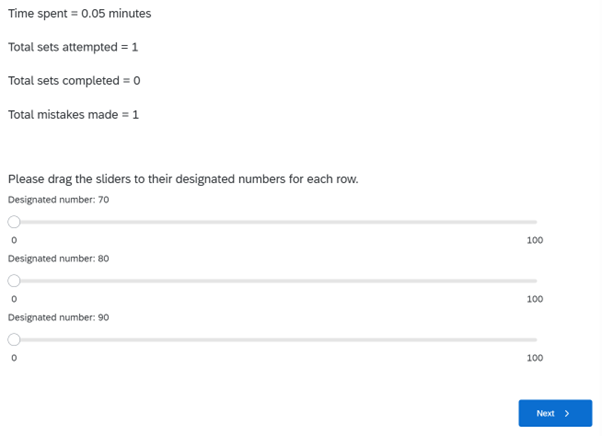
\includegraphics[width=0.75\linewidth]{survey_screenshots/slider_task_set_example.png}
\caption{Example of a set in the slider task}\label{fig-slider-set-example}
\end{figure}

The slider task was selected because it is mundane and repetitive, hence reasonably incurring a positive effort cost. This combined with the fact that working on the task provides no intrinsic value should make it inert to variation in personal motivation regarding the task. The task is also easy and intuitive so task performance will be less affected by differences in intelligence and education/ training among subjects, and more clearly maps from effort exertion. These will help to reduce noise in the effort measures. The task is also intentionally abstract in nature and generic in its assessment since this study seeks to find universal decision-making processes regarding effort exertion under reference point effects which has generalisability to a broad range of jobs and possibly even beyond the labour supply domain. The short task duration and low stakes may be unrealistic compared to long-term jobs, but have to be imposed for practical reasons, and still offers insight into how people respond to multi-dimensional targets at the task level of a job (e.g.~a single ride for an Uber driver), which can plausibly be aggregated to the job level. Overall, the objective is not to exactly capture how people work under targets in specific jobs, but identify fundamental decision-making mechanisms which can apply to various domains and vary across them as permitted by the parameters in the model.

There were four treatment groups which varied the task parameters in terms of the reference points (i.e.~targets) and how the work was assessed. Reference points were set in the two performance dimensions: speed as measured by the number of sets completed, and accuracy as measured by the proportion of \emph{recorded} mistakes out of sets attempted. Work was assessed by either of two criteria: strict which records all actual mistakes made, and lenient which records only a quarter. The probability for each criterion differs across treatments. Subjects who are more likely to be assessed by a strict criterion thus have a lower likelihood of achieving both reference points concurrently. To reinforce this perception, subjects were primed to think that ``achieving both targets [was] manageable under a lenient criterion but highly challenging under a strict criterion''. Reference points were also either presented as is or explained in greater detail by explicating how performance in the speed dimension relates to that in the accuracy dimension. The explanation constituted a table showing the maximum number of total actual mistakes allowed under each criterion for different number of total tasks completed. This was intended to reduce the cognitive complexity of reconciling both reference points.

Treatment 1 was the control group with no reference points which were assessed by the strict criterion for sure; subjects in this group were unaware about the different assessment criteria. Treatments 2, 3, and 4 were the treated groups which were set the same reference points: at least 45 sets completed in 5 minutes and at most 10\% recorded mistakes\footnote{These targets were calibrated from an initial trial of the task, such that achieving both targets under the strict criterion had zero probability in the empirical distrbution but 50\% probability under the lenient criterion. Subjects were from my social circle and requested to do as many sets and as accurately they could.}. Treatments 2 and 4 had a 75\% probability of getting a lenient assessment criterion and 25\% probability of strict, whereas treatment 3 had the inverse. Treatments 2 and 3 had the reference points explained in greater detail, whereas treatment 4 did not. The control allows for verification of the existence of reference point effects, which is a prerequisite to identifying changes in those effects due to treatment. Comparing treatments 2 and 3 demonstrates the role of probabilistic expectations of concurrent achievement of targets in attenuating reference point effects, whereas comparing treatments 2 and 4 elicits the role of cognitive complexity. Table~\ref{tbl-treatment-groups} summarises the four treatment groups and their treatment conditions. Common instructions for the experiment and specific ones for each treatment group are attached in Appendix A4. Subjects in the treated groups were required to pass a comprehension check (also attached in Appendix A4) before proceeding onto the actual task.

\bigskip

\begin{longtable}[]{@{}
  >{\raggedright\arraybackslash}p{(\linewidth - 6\tabcolsep) * \real{0.1222}}
  >{\raggedright\arraybackslash}p{(\linewidth - 6\tabcolsep) * \real{0.2000}}
  >{\raggedright\arraybackslash}p{(\linewidth - 6\tabcolsep) * \real{0.5000}}
  >{\raggedright\arraybackslash}p{(\linewidth - 6\tabcolsep) * \real{0.1778}}@{}}
\toprule
Treatment & Reference Points & Assessment Criteria Probabilities & Explanation \\
\midrule
\endhead
\bottomrule
\caption{Treatment groups and conditions}\label{tbl-treatment-groups}
\endlastfoot
1 & No & 100\% strict & Not applicable \\
2 & Yes & 25\% chance of strict, 75\% chance of lenient & Yes \\
3 & Yes & 75\% chance of strict, 25\% chance of lenient & Yes \\
4 & Yes & 25\% chance of strict, 75\% chance of lenient & No \\
\end{longtable}

After the task, all subjects were requested to complete an optional questionnaire on their charcateristics and reflections on the task. Characteristics collected include gender, race, age, household income, education level, study of economics at the undergraduate level or higher, mouse usage in the task, occupational type, and loss aversion levels. Loss aversion levels were solicited by asking subjects to indicate the number of correctly completed sets they were willing to do under different payment structures: half of them paid a fixed piece rate and the other half paid either a high or low piece rate with equal probabilities, and each fixed piece rate was paired with a random piece rate of the same expected payment value; this was in line with \textcite{campos-mercade.2024.gustibusdisputes}. The fixed and random piece rates were presented on separate pages, and the order of the pages and the piece rates within each page were randomised to negate any order effects. The characteristics collected represent factors which may affect task performance aside from exert exertion. Thus, I could check for balance of these characteristics between treatment groups, control for them if imbalance is found (or even if not as they can improve precision of estimates), and examine which may drive differential responses to the treatment so I can conduct heterogeneity analysis. Reflections on the task asked about subjects' goals for speed and accuracy, whether they attempted to achieve the set targets, and if not their reasons for ignoring the targets, which provided a qualitative check of how they interpreted the reference points and treatment conditions.

Samples were drawn from two populations: undergraduate students at the \emph{University of Chicago} recruited through the instructors of specific courses, and the general public of Chicago recruited through the research laboratories of the \emph{Roman Family Center for Decision Research} (RFCDR) at the \emph{University of Chicago's Booth School of Business}. Treatment assignment was stratified on the three subsamples: \emph{10000 Principles of Microeconomics} students, \emph{10200 Principles of Macroeconomics} students, and RFCDR lab participants. I anticipate concerns about the external validity of the study due to sampling biases. The RFCDR lab sample would be more representative of the general population, but due to funding restrictions, I could only run my experiment with 200 subjects, which may be insufficient to identify treatment effects \footnote{Preliminary power analysis indicated an upper bound sample size requirement of 179 observations per treatment group (716 observations total) given a conservative estimate of the minimum detectable effect size (Pearson's r) of 0.24 standard deviations and equal outcome variances across groups.}. The undergraduate student sample was chosen as a cost-free way to supplement sample size, even though they may be less representative of how the average person thinks and acts. Another concern is that RFCDR lab subjects also suffer selection bias as the composition of people who are exposed and responsive to the organisation could differ from those who are in the general population (e.g.~wealthier, more educated, greater interest and familiarity with behavioral research etc). Moreover, the composition of people who elect into the study may differ from those who do not (e.g.~more risk-averse, more leisure time, more motivated towards knowledge creation etc). However, in the same vein of reasoning above, I would argue that the experiment investigates general decision-making processes which has broad transference across populations, though it would be important check for differences in responses between the subsamples.

To incentivise participation, those from the undergraduate student sample were offered a fixed amount of course credit (0.5\% for the microeconomics class and 1\% for the macroeconomics class) for completing the study, whereas those from the general public sample were offered a flat fee for participation (technically payment is pro-rated based on time spent at \$1 per 5 minutes but task duration and hence compensation for just the task alone is fixed). Ideally, there would have been additional incentives (beyond intrinsic motivation from the targets) for effort exertion in the task to better parallel economic settings. However, this was not feasible in the student sample due to fairness concerns as awarding additional class credit based on task performance would depend on the assessment criteria which was assigned by chance, nor in the lab sample due to budgetary constraints (otherwise it would have further shrunk the sample size). Again, this may cause selection issues; \textcite{harrison.2009.riskattitudes} evinced that a fixed payment for participation can attract more risk-averse people, so this will be important to keep in mind when evaluating treatment effects.

Participants completed the experiment virtually on Qualtrics. Conducting the experiment in-person would have afforded greater control over the task environment and hence reduced noise in effort measures, but given the time constraints, I opted for an online mode to improve accessibility so that I could more quickly collect sufficient data. Furthermore, conducting the experiment in-person was particularly difficult to operationalise for students, as I needed to conduct the experiment outside of class time which was difficult to organise given the different schedules of the students. This would have necessitated running the experiment on several occasions and obtaining permission to use university facilities each time. While implementation was more viable at the RFCDR labs, it was better to standardise the experiment medium for better comparability across the two subject pools since that was the main purpose of supplementing the lab sample with the student sample.

Treatment assignment is completely randomised at the individual subject level within each subsample and equally split\footnote{This is slightly different from the optimal sample size split, but that was based on calculations extrapolated from a different experiment which may not be strongly founded in this context, plus unequal sample size allocation was harder to operationalise, and the differences were not too large, hence I opted for an equal allocation. The optimal sample size split calculations can be found in Appendix A3.} between the four treatment groups. A stratified randomisation based on covariates would have been preferred to mitigate against possible covariate imbalance between treatment groups which can occur chance, with an optimal matched pair design minimising the mean-squared error of treatment effect estimates conditional on covariates \parencite{bai.2022.optimalitymatchedpair}. However, this would have required collection of covariate data pre-treatment for matching. Instead, I had resorted to acquiring this information through a post-task questionnaire which was optional and unincentivised due to budgetary constraints. It was likely that imposing such a requirement pre-task without additional incentives would have deterred participation and had a counterproductive effect on statistical inferential power and precision. However, with sufficient finances to incentivise and time to conduct a pre-treatment survey, I would have adopted stratified randomisation by blocking on key covariates such as gender, age, whether the subject studied economics at the undergraduate level or above, occupational type, and loss aversion level.

\subsection{Theoretical specification and hypotheses}\label{theoretical-specification-and-hypotheses}

I develop refinements to the KR model to capture the effect of probabilistic expectations and cognitive complexity in reference-dependence, which produce distinct testable predictions for the experiment.

In the experiment, the agent works on a task where he/she has to exert effort \(e\), and has targets \(N\) for the number of tasks completed per minute, and \(Q\) for the percentage of \emph{actual} mistakes. \(e\) is split into \(e_1\), effort in speed, and \(e_2\), effort in accuracy. First, consider a simplified version where outcomes are deterministic, reference points are degenerate, and gain-loss utilities are linear with constant loss aversion. Under the KR model, expected utility from effort across two dimensions is given by the KR model as
\[
\begin{aligned}
U = & p(e_1, e_2) - c(e_1, e_2) + \nonumber \\
    & \mu_1[(n(e_1)-N)\mathbb{I}(n \geq N) + \lambda_1(n(e_1)-N)\mathbb{I}(n<N)] + \nonumber \\
    & \mu_2[(Q-q(e_2))\mathbb{I}(q \leq Q) + \lambda_2(Q-q(e_2))\mathbb{I}(q>Q)]
\end{aligned}
\]
\(p(e)\) is the level payoff from effort exertion, summed across both dimensions. \(c(e)\) is the cost of effort. \(\mu_1[(n(e_1)-N)\mathbb{I}(n \geq N) + \lambda_1(n(e_1)-N)\mathbb{I}(n<N)]\) is the gain-loss utility in the speed dimension, where \(\mu_1 \geq 0\) is the gain-loss parameter, \(\lambda \geq 1\) is the loss aversion parameter, and \(\mathbb{I}(.)\) is an indicator function equaling 1 when the condition in the bracket holds and 0 otherwise. \(\mu_2 [(Q-q(e_2))\mathbb{I}(q \leq Q) + \lambda_2(Q-q(e_2))\mathbb{I}(q>Q)])]\) is analogously defined for the accuracy dimension.

To account for the role of probabilistic expectations and cognitive complexity in reference point effects, I propose the appended model
\[
\begin{aligned}
U = & p(e_1, e_2) - c(e_1, e_2) + \nonumber \\
    & E[\mathbb{P}(\{n \geq N - \varepsilon \} \cap \{q \leq Q + \varepsilon\})] \times \theta \times & \{\mu_1[(n(e_1 )-N)\mathbb{I}(n \geq N) + \lambda_1(n(e_1)-N)\mathbb{I}(n<N)] + \nonumber \\
    && \mu_2[(Q-q(e_2))\mathbb{I}(q \leq Q) + \lambda_2(Q-q(e_2))\mathbb{I}(q>Q)]\}
\end{aligned}
\]
The first additional term \(E[\mathbb{P}(\{n \geq N - \varepsilon \} \cap \{q \leq Q + \varepsilon\}]\) captures the agent's expected probability of simultaneously achieving (within some bandwidth \(\varepsilon\) of) the reference points. When this expected probability is lower, the agent weights the gain-loss utilities less and hence is less responsive to the reference points. The second additional parameter \(\theta \geq 0\) is a parameter decreasing in the cognitive complexity required to integrate the multiple reference points, so greater cognitive complexity attenuates reference point effects.

Extending the model to the context of the slider task with strict and lenient assessment criteria, we have
\[
\begin{aligned}
U = & p(e_1, e_2) - c(e_1, e_2) + \nonumber \\
    & \mathbb{P}^E \times \theta \times [\phi_1(\mu_1, \lambda_1, n(e_1), N) + \phi_2(\mu_2, \lambda_2, n(e_2), Q)] \nonumber \\
\text{Where}
\\
\phi_1 = & \mu_1[(n(e_1)-N)\mathbb{I}(n \geq N) + \lambda_1(n(e_1)-N)\mathbb{I}(n<N)] \nonumber \\
\phi_2 = & \mu_2 \{P_s[(Q-q(e_2))\mathbb{I}(q \leq Q) + \lambda_2(Q-q(e_2))\mathbb{I}(q>Q)] + \nonumber \\
& \qquad P_l[(4Q-q(e_2))\mathbb{I}(q \leq Q) + \lambda_2(4Q-q(e_2))\mathbb{I}(q>Q)]\}
\end{aligned}
\]
\(\mathbb{P}^E\) is the expected probability term from before, \(P_s\) is the probability of getting a strict assessment criteria, and \(P-l\) is the probability of getting a leninet criteria. Differentiating with respect to effort, the two models provide distinct predictions for optimal effort provision in the real effort experiment\footnote{Appendix A2 for formal derivation of the first-order conditions.}. Essentially, without accounting for the role of probabilistic expectations and cognitive complexity, the KR model predicts that subjects would respond to a higher chance of being assessed by a strict criteria by reducing actual mistakes made since they are more likely to be recorded, exerting more effort in the accuracy dimension either in addition to effort in the speed dimension or at the expense of it, and subjects' responsiveness to the targets are not affected by whether there is an explanation of how the two performance dimensions and their targets are related. Conversely, the appended model predicts that subjects faced with a higher chance of being assessed by a strict criteria would exert less effort in both performance dimensions since they believe it less likely to achieve them and hence attenuate them, and subjects provided with an explanation would exert more effort in both performance dimensions since they are better able to reconcile the targets to inform their effort exertion choices and hence act more responsively to the targets. These produce testable hypotheses about the treatment effects, holding the assessment criteria constant.

\noindent KR model predictions:

\begin{itemize}
\tightlist
\item
  KR1: Treatments 2 and 4 will have similar positive effects on the probability of achieving any target.
\item
  KR2: Treatment 3 should have a larger positive effect than treatments 2 and 4 for achieving the accuracy target and either equal or lower positive effect for achieving the speed target.
\end{itemize}

\noindent Appended model predictions:

\begin{itemize}
\tightlist
\item
  A1: Treatment 3 will have lower positive effect for achieving any target than treatment 2, and in the extreme tend to treatment 1 (no effect).
\item
  A2: Treatment 4 will have a lower positive effect for achieving any targets than treatment 2, and in the extreme tend to treatment 1 (no effect).
\end{itemize}

\section{Data}\label{data}

The experiment garnered a total of \NumObs{} observations\footnote{I only include participants who completed the study. Including those who did not, there were \NumRespondents{} respondents.} with \NumObsLab{} from the RFCDR labs and \NumObsClass{} from the undergraduate economics classes: \NumObsMicro{} in microeconomics and \NumObsMacro{} in macroeconomics. Overall, the sample is roughly equally divided between the three sources.

\begin{table}
\centering
{\fontsize{9.0pt}{11.0pt}\selectfont
\begin{tabular*}{\linewidth}{@{\extracolsep{\fill}}>{\raggedright\arraybackslash}p{\dimexpr 131.25pt -2\tabcolsep-1.5\arrayrulewidth}ccccc>{\centering\arraybackslash}p{\dimexpr 37.50pt -2\tabcolsep-1.5\arrayrulewidth}>{\centering\arraybackslash}p{\dimexpr 37.50pt -2\tabcolsep-1.5\arrayrulewidth}}
\toprule
 &  & \multicolumn{4}{c}{\textbf{Treatments}} &  &  \\ 
\cmidrule(lr){3-6}
\textbf{Metric} & \textbf{All}\textsuperscript{\textit{1}} & \textbf{1}\textsuperscript{\textit{1}} & \textbf{2}\textsuperscript{\textit{1}} & \textbf{3}\textsuperscript{\textit{1}} & \textbf{4}\textsuperscript{\textit{1}} & \textbf{p-value}\textsuperscript{\textit{2,3}} & \textbf{p-value}\textsuperscript{\textit{3,4}} \\ 
\midrule\addlinespace[2.5pt]
{\bfseries Gender} &  &  &  &  &  & >0.9 & >0.9 \\ 
    Male & 63 (30\%) & 17 (29\%) & 14 (29\%) & 16 (31\%) & 16 (32\%) &  &  \\ 
    Female & 140 (67\%) & 40 (69\%) & 32 (67\%) & 35 (67\%) & 33 (66\%) &  &  \\ 
    Non-binary & 5 (2.4\%) & 1 (1.7\%) & 2 (4.2\%) & 1 (1.9\%) & 1 (2.0\%) &  &  \\ 
{\bfseries Race} &  &  &  &  &  & 0.050 & 0.14 \\ 
    White & 92 (45\%) & 25 (43\%) & 25 (52\%) & 21 (40\%) & 21 (44\%) &  &  \\ 
    Asian & 68 (33\%) & 13 (22\%) & 18 (38\%) & 18 (35\%) & 19 (40\%) &  &  \\ 
    Black & 24 (12\%) & 10 (17\%) & 0 (0\%) & 9 (17\%) & 5 (10\%) &  &  \\ 
    Hispanic & 16 (7.8\%) & 7 (12\%) & 3 (6.3\%) & 3 (5.8\%) & 3 (6.3\%) &  &  \\ 
    Mixed & 6 (2.9\%) & 3 (5.2\%) & 2 (4.2\%) & 1 (1.9\%) & 0 (0\%) &  &  \\ 
{\bfseries Age} & 30 (11) & 30 (12) & 31 (13) & 30 (11) & 28 (8) & 0.8 & 0.6 \\ 
{\bfseries Household Income} &  &  &  &  &  & 0.7 & 0.7 \\ 
    0 - 24,999 & 46 (23\%) & 12 (22\%) & 12 (27\%) & 8 (16\%) & 14 (29\%) &  &  \\ 
    25,000 - 49,999 & 34 (17\%) & 11 (20\%) & 4 (9.1\%) & 9 (18\%) & 10 (21\%) &  &  \\ 
    50,000 - 74,999 & 34 (17\%) & 9 (16\%) & 9 (20\%) & 11 (22\%) & 5 (10\%) &  &  \\ 
    75,000 - 119,999 & 32 (16\%) & 9 (16\%) & 5 (11\%) & 10 (20\%) & 8 (17\%) &  &  \\ 
    120,000 - 199,999 & 28 (14\%) & 6 (11\%) & 10 (23\%) & 7 (14\%) & 5 (10\%) &  &  \\ 
    200,000 and over & 22 (11\%) & 8 (15\%) & 4 (9.1\%) & 4 (8.2\%) & 6 (13\%) &  &  \\ 
{\bfseries Education Level} &  &  &  &  &  & 0.4 & 0.4 \\ 
    Below high school diploma & 1 (0.5\%) & 0 (0\%) & 1 (2.2\%) & 0 (0\%) & 0 (0\%) &  &  \\ 
    High school diploma & 41 (20\%) & 11 (19\%) & 12 (26\%) & 7 (13\%) & 11 (22\%) &  &  \\ 
    College degree or above & 163 (80\%) & 47 (81\%) & 33 (72\%) & 45 (87\%) & 38 (78\%) &  &  \\ 
{\bfseries Studied Economics} & 58 (28\%) & 18 (31\%) & 10 (21\%) & 22 (42\%) & 8 (16\%) & 0.017* & 0.017* \\ 
{\bfseries Occupation} &  &  &  &  &  & 0.6 & 0.5 \\ 
    Student & 72 (36\%) & 22 (39\%) & 20 (43\%) & 15 (31\%) & 15 (31\%) &  &  \\ 
    Academia & 30 (15\%) & 6 (11\%) & 6 (13\%) & 6 (12\%) & 12 (24\%) &  &  \\ 
    Clerical & 13 (6.5\%) & 2 (3.6\%) & 4 (8.5\%) & 6 (12\%) & 1 (2.0\%) &  &  \\ 
    High-tech mfg or eng & 11 (5.5\%) & 2 (3.6\%) & 1 (2.1\%) & 2 (4.1\%) & 6 (12\%) &  &  \\ 
    Managerial & 13 (6.5\%) & 4 (7.1\%) & 3 (6.4\%) & 3 (6.1\%) & 3 (6.1\%) &  &  \\ 
    Professional services & 45 (22\%) & 13 (23\%) & 9 (19\%) & 13 (27\%) & 10 (20\%) &  &  \\ 
    Unemployed & 11 (5.5\%) & 4 (7.1\%) & 2 (4.3\%) & 3 (6.1\%) & 2 (4.1\%) &  &  \\ 
    Other & 6 (3.0\%) & 3 (5.4\%) & 2 (4.3\%) & 1 (2.0\%) & 0 (0\%) &  &  \\ 
{\bfseries Used Mouse} & 122 (58\%) & 33 (55\%) & 31 (63\%) & 31 (60\%) & 27 (54\%) & 0.8 & 0.8 \\ 
\bottomrule
\end{tabular*}
\begin{minipage}{\linewidth}
\textsuperscript{\textit{1}}n (\%); Mean (SD)\\
\textsuperscript{\textit{2}}Fisher's Exact Test for Count Data with simulated p-value
(based on 10000 replicates); Kruskal-Wallis rank sum test\\
\textsuperscript{\textit{3}}*p\textless{}0.05; **p\textless{}0.01; ***p\textless{}0.001\\
\textsuperscript{\textit{4}}Pearson's Chi-squared test; One-way analysis of means (not assuming equal variances)\\
\end{minipage}
\par}
\caption{Covariate balance for lab sample}\label{tbl-covariates-sumstats-lab}
\end{table}

\begin{table}
\centering
{\fontsize{9.0pt}{11.0pt}\selectfont
\begin{tabular*}{\linewidth}{@{\extracolsep{\fill}}>{\raggedright\arraybackslash}p{\dimexpr 131.25pt -2\tabcolsep-1.5\arrayrulewidth}>{\centering\arraybackslash}p{\dimexpr 56.25pt -2\tabcolsep-1.5\arrayrulewidth}>{\centering\arraybackslash}p{\dimexpr 56.25pt -2\tabcolsep-1.5\arrayrulewidth}>{\centering\arraybackslash}p{\dimexpr 56.25pt -2\tabcolsep-1.5\arrayrulewidth}>{\centering\arraybackslash}p{\dimexpr 56.25pt -2\tabcolsep-1.5\arrayrulewidth}>{\centering\arraybackslash}p{\dimexpr 56.25pt -2\tabcolsep-1.5\arrayrulewidth}>{\centering\arraybackslash}p{\dimexpr 37.50pt -2\tabcolsep-1.5\arrayrulewidth}>{\centering\arraybackslash}p{\dimexpr 37.50pt -2\tabcolsep-1.5\arrayrulewidth}}
\toprule
 &  & \multicolumn{4}{c}{\textbf{Treatments}} &  &  \\ 
\cmidrule(lr){3-6}
\textbf{Metric} & \textbf{All}\textsuperscript{\textit{1}} & \textbf{1}\textsuperscript{\textit{1}} & \textbf{2}\textsuperscript{\textit{1}} & \textbf{3}\textsuperscript{\textit{1}} & \textbf{4}\textsuperscript{\textit{1}} & \textbf{p-value}\textsuperscript{\textit{2,3}} & \textbf{p-value}\textsuperscript{\textit{3,4}} \\ 
\midrule\addlinespace[2.5pt]
{\bfseries Gender} &  &  &  &  &  & 0.2 & 0.2 \\ 
    Male & 139 (62\%) & 40 (66\%) & 28 (54\%) & 39 (72\%) & 32 (54\%) &  &  \\ 
    Female & 86 (38\%) & 21 (34\%) & 24 (46\%) & 15 (28\%) & 26 (44\%) &  &  \\ 
    Non-binary & 1 (0.4\%) & 0 (0\%) & 0 (0\%) & 0 (0\%) & 1 (1.7\%) &  &  \\ 
{\bfseries Race} &  &  &  &  &  & >0.9 & >0.9 \\ 
    White & 82 (37\%) & 25 (41\%) & 15 (29\%) & 19 (37\%) & 23 (40\%) &  &  \\ 
    Asian & 92 (41\%) & 23 (38\%) & 26 (50\%) & 21 (40\%) & 22 (38\%) &  &  \\ 
    Black & 15 (6.7\%) & 3 (4.9\%) & 3 (5.8\%) & 4 (7.7\%) & 5 (8.6\%) &  &  \\ 
    Hispanic & 22 (9.9\%) & 7 (11\%) & 5 (9.6\%) & 5 (9.6\%) & 5 (8.6\%) &  &  \\ 
    Mixed & 12 (5.4\%) & 3 (4.9\%) & 3 (5.8\%) & 3 (5.8\%) & 3 (5.2\%) &  &  \\ 
{\bfseries Age} & 19.89 (1.15) & 19.93 (1.53) & 20.00 (1.13) & 19.88 (0.85) & 19.76 (0.92) & 0.7 & 0.7 \\ 
{\bfseries Household Income} &  &  &  &  &  & 0.6 & 0.7 \\ 
    0 - 24,999 & 12 (6.1\%) & 5 (8.9\%) & 3 (6.7\%) & 1 (2.1\%) & 3 (6.1\%) &  &  \\ 
    25,000 - 49,999 & 9 (4.6\%) & 0 (0\%) & 4 (8.9\%) & 3 (6.4\%) & 2 (4.1\%) &  &  \\ 
    50,000 - 74,999 & 10 (5.1\%) & 3 (5.4\%) & 2 (4.4\%) & 3 (6.4\%) & 2 (4.1\%) &  &  \\ 
    75,000 - 119,999 & 21 (11\%) & 7 (13\%) & 4 (8.9\%) & 2 (4.3\%) & 8 (16\%) &  &  \\ 
    120,000 - 199,999 & 26 (13\%) & 9 (16\%) & 4 (8.9\%) & 7 (15\%) & 6 (12\%) &  &  \\ 
    200,000 and over & 119 (60\%) & 32 (57\%) & 28 (62\%) & 31 (66\%) & 28 (57\%) &  &  \\ 
{\bfseries Used Mouse} & 71 (31\%) & 19 (30\%) & 15 (28\%) & 19 (37\%) & 18 (30\%) & 0.8 & 0.8 \\ 
\bottomrule
\end{tabular*}
\begin{minipage}{\linewidth}
\textsuperscript{\textit{1}}n (\%); Mean (SD)\\
\textsuperscript{\textit{2}}Fisher's Exact Test for Count Data with simulated p-value
(based on 10000 replicates); Kruskal-Wallis rank sum test\\
\textsuperscript{\textit{3}}*p\textless{}0.05; **p\textless{}0.01; ***p\textless{}0.001\\
\textsuperscript{\textit{4}}Pearson's Chi-squared test; One-way analysis of means (not assuming equal variances)\\
\end{minipage}
\par}
\caption{Covariate balance for microeconomic class sample}\label{tbl-covariates-sumstats-micro}
\end{table}

\begin{table}
\centering
{\fontsize{9.0pt}{11.0pt}\selectfont
\begin{tabular*}{\linewidth}{@{\extracolsep{\fill}}>{\raggedright\arraybackslash}p{\dimexpr 131.25pt -2\tabcolsep-1.5\arrayrulewidth}>{\centering\arraybackslash}p{\dimexpr 56.25pt -2\tabcolsep-1.5\arrayrulewidth}>{\centering\arraybackslash}p{\dimexpr 56.25pt -2\tabcolsep-1.5\arrayrulewidth}>{\centering\arraybackslash}p{\dimexpr 56.25pt -2\tabcolsep-1.5\arrayrulewidth}>{\centering\arraybackslash}p{\dimexpr 56.25pt -2\tabcolsep-1.5\arrayrulewidth}>{\centering\arraybackslash}p{\dimexpr 56.25pt -2\tabcolsep-1.5\arrayrulewidth}>{\centering\arraybackslash}p{\dimexpr 37.50pt -2\tabcolsep-1.5\arrayrulewidth}>{\centering\arraybackslash}p{\dimexpr 37.50pt -2\tabcolsep-1.5\arrayrulewidth}}
\toprule
 &  & \multicolumn{4}{c}{\textbf{Treatments}} &  &  \\ 
\cmidrule(lr){3-6}
\textbf{Metric} & \textbf{All}\textsuperscript{\textit{1}} & \textbf{1}\textsuperscript{\textit{1}} & \textbf{2}\textsuperscript{\textit{1}} & \textbf{3}\textsuperscript{\textit{1}} & \textbf{4}\textsuperscript{\textit{1}} & \textbf{p-value}\textsuperscript{\textit{2,3}} & \textbf{p-value}\textsuperscript{\textit{3,4}} \\ 
\midrule\addlinespace[2.5pt]
{\bfseries Gender} &  &  &  &  &  & 0.6 & 0.6 \\ 
    Male & 97 (52\%) & 22 (44\%) & 22 (49\%) & 24 (60\%) & 29 (56\%) &  &  \\ 
    Female & 88 (47\%) & 27 (54\%) & 23 (51\%) & 16 (40\%) & 22 (42\%) &  &  \\ 
    Non-binary & 2 (1.1\%) & 1 (2.0\%) & 0 (0\%) & 0 (0\%) & 1 (1.9\%) &  &  \\ 
{\bfseries Race} &  &  &  &  &  & 0.4 & 0.4 \\ 
    White & 62 (34\%) & 20 (42\%) & 12 (27\%) & 11 (28\%) & 19 (39\%) &  &  \\ 
    Asian & 77 (43\%) & 19 (40\%) & 23 (51\%) & 17 (44\%) & 18 (37\%) &  &  \\ 
    Black & 13 (7.2\%) & 5 (10\%) & 2 (4.4\%) & 5 (13\%) & 1 (2.0\%) &  &  \\ 
    Hispanic & 21 (12\%) & 3 (6.3\%) & 6 (13\%) & 5 (13\%) & 7 (14\%) &  &  \\ 
    Mixed & 8 (4.4\%) & 1 (2.1\%) & 2 (4.4\%) & 1 (2.6\%) & 4 (8.2\%) &  &  \\ 
{\bfseries Age} & 20.13 (2.00) & 19.72 (2.88) & 20.24 (1.12) & 20.49 (2.27) & 20.13 (1.08) & 0.9 & 0.6 \\ 
{\bfseries Household Income} &  &  &  &  &  & 0.5 & 0.5 \\ 
    0 - 24,999 & 11 (6.6\%) & 5 (12\%) & 2 (4.9\%) & 1 (2.6\%) & 3 (6.7\%) &  &  \\ 
    25,000 - 49,999 & 4 (2.4\%) & 0 (0\%) & 1 (2.4\%) & 1 (2.6\%) & 2 (4.4\%) &  &  \\ 
    50,000 - 74,999 & 7 (4.2\%) & 2 (4.8\%) & 3 (7.3\%) & 2 (5.3\%) & 0 (0\%) &  &  \\ 
    75,000 - 119,999 & 15 (9.0\%) & 6 (14\%) & 4 (9.8\%) & 1 (2.6\%) & 4 (8.9\%) &  &  \\ 
    120,000 - 199,999 & 23 (14\%) & 5 (12\%) & 8 (20\%) & 6 (16\%) & 4 (8.9\%) &  &  \\ 
    200,000 and over & 106 (64\%) & 24 (57\%) & 23 (56\%) & 27 (71\%) & 32 (71\%) &  &  \\ 
{\bfseries Used Mouse} & 59 (32\%) & 16 (30\%) & 14 (33\%) & 11 (28\%) & 18 (35\%) & 0.9 & 0.9 \\ 
\bottomrule
\end{tabular*}
\begin{minipage}{\linewidth}
\textsuperscript{\textit{1}}n (\%); Mean (SD)\\
\textsuperscript{\textit{2}}Fisher's Exact Test for Count Data with simulated p-value
(based on 10000 replicates); Kruskal-Wallis rank sum test\\
\textsuperscript{\textit{3}}*p\textless{}0.05; **p\textless{}0.01; ***p\textless{}0.001\\
\textsuperscript{\textit{4}}Pearson's Chi-squared test; One-way analysis of means (not assuming equal variances)\\
\end{minipage}
\par}
\caption{Covariate balance for macroeconomic class sample}\label{tbl-covariates-sumstats-macro}
\end{table}

\begin{table}
\centering
{\fontsize{9.0pt}{11.0pt}\selectfont
\begin{tabular*}{\linewidth}{@{\extracolsep{\fill}}>{\raggedright\arraybackslash}p{\dimexpr 131.25pt -2\tabcolsep-1.5\arrayrulewidth}ccccc>{\centering\arraybackslash}p{\dimexpr 37.50pt -2\tabcolsep-1.5\arrayrulewidth}>{\centering\arraybackslash}p{\dimexpr 37.50pt -2\tabcolsep-1.5\arrayrulewidth}}
\toprule
 &  & \multicolumn{4}{c}{\textbf{Treatments}} &  &  \\ 
\cmidrule(lr){3-6}
\textbf{Metric} & \textbf{All}\textsuperscript{\textit{1}} & \textbf{1}\textsuperscript{\textit{1}} & \textbf{2}\textsuperscript{\textit{1}} & \textbf{3}\textsuperscript{\textit{1}} & \textbf{4}\textsuperscript{\textit{1}} & \textbf{p-value}\textsuperscript{\textit{2,3}} & \textbf{p-value}\textsuperscript{\textit{3,4}} \\ 
\midrule\addlinespace[2.5pt]
{\bfseries Gender} &  &  &  &  &  & 0.7 & 0.7 \\ 
    Male & 299 (48\%) & 79 (47\%) & 64 (44\%) & 79 (54\%) & 77 (48\%) &  &  \\ 
    Female & 314 (51\%) & 88 (52\%) & 79 (54\%) & 66 (45\%) & 81 (50\%) &  &  \\ 
    Non-binary & 8 (1.3\%) & 2 (1.2\%) & 2 (1.4\%) & 1 (0.7\%) & 3 (1.9\%) &  &  \\ 
{\bfseries Race} &  &  &  &  &  & 0.3 & 0.3 \\ 
    White & 236 (39\%) & 70 (42\%) & 52 (36\%) & 51 (36\%) & 63 (41\%) &  &  \\ 
    Asian & 237 (39\%) & 55 (33\%) & 67 (46\%) & 56 (39\%) & 59 (38\%) &  &  \\ 
    Black & 52 (8.5\%) & 18 (11\%) & 5 (3.4\%) & 18 (13\%) & 11 (7.1\%) &  &  \\ 
    Hispanic & 59 (9.7\%) & 17 (10\%) & 14 (9.7\%) & 13 (9.1\%) & 15 (9.7\%) &  &  \\ 
    Mixed & 26 (4.3\%) & 7 (4.2\%) & 7 (4.8\%) & 5 (3.5\%) & 7 (4.5\%) &  &  \\ 
{\bfseries Age} & 23 (8) & 23 (9) & 24 (9) & 24 (8) & 23 (6) & 0.3 & 0.5 \\ 
{\bfseries Household Income} &  &  &  &  &  & 0.5 & 0.5 \\ 
    0 - 24,999 & 69 (12\%) & 22 (14\%) & 17 (13\%) & 10 (7.5\%) & 20 (14\%) &  &  \\ 
    25,000 - 49,999 & 47 (8.4\%) & 11 (7.2\%) & 9 (6.9\%) & 13 (9.7\%) & 14 (9.9\%) &  &  \\ 
    50,000 - 74,999 & 51 (9.1\%) & 14 (9.2\%) & 14 (11\%) & 16 (12\%) & 7 (4.9\%) &  &  \\ 
    75,000 - 119,999 & 68 (12\%) & 22 (14\%) & 13 (10\%) & 13 (9.7\%) & 20 (14\%) &  &  \\ 
    120,000 - 199,999 & 77 (14\%) & 20 (13\%) & 22 (17\%) & 20 (15\%) & 15 (11\%) &  &  \\ 
    200,000 and over & 247 (44\%) & 64 (42\%) & 55 (42\%) & 62 (46\%) & 66 (46\%) &  &  \\ 
{\bfseries Education Level} &  &  &  &  &  & 0.6 & 0.6 \\ 
    Below high school diploma & 1 (0.2\%) & 0 (0\%) & 1 (0.7\%) & 0 (0\%) & 0 (0\%) &  &  \\ 
    High school diploma & 41 (6.5\%) & 11 (6.3\%) & 12 (8.2\%) & 7 (4.7\%) & 11 (6.7\%) &  &  \\ 
    College degree or above & 592 (93\%) & 165 (94\%) & 133 (91\%) & 141 (95\%) & 153 (93\%) &  &  \\ 
{\bfseries Studied Economics} & 487 (77\%) & 136 (77\%) & 110 (75\%) & 118 (80\%) & 123 (75\%) & 0.7 & 0.7 \\ 
{\bfseries Occupation} &  &  &  &  &  & 0.7 & 0.6 \\ 
    Student & 501 (80\%) & 140 (80\%) & 120 (82\%) & 111 (77\%) & 130 (79\%) &  &  \\ 
    Academia & 30 (4.8\%) & 6 (3.4\%) & 6 (4.1\%) & 6 (4.1\%) & 12 (7.3\%) &  &  \\ 
    Clerical & 13 (2.1\%) & 2 (1.1\%) & 4 (2.7\%) & 6 (4.1\%) & 1 (0.6\%) &  &  \\ 
    High-tech mfg or eng & 11 (1.7\%) & 2 (1.1\%) & 1 (0.7\%) & 2 (1.4\%) & 6 (3.7\%) &  &  \\ 
    Managerial & 13 (2.1\%) & 4 (2.3\%) & 3 (2.0\%) & 3 (2.1\%) & 3 (1.8\%) &  &  \\ 
    Professional services & 45 (7.1\%) & 13 (7.5\%) & 9 (6.1\%) & 13 (9.0\%) & 10 (6.1\%) &  &  \\ 
    Unemployed & 11 (1.7\%) & 4 (2.3\%) & 2 (1.4\%) & 3 (2.1\%) & 2 (1.2\%) &  &  \\ 
    Other & 6 (1.0\%) & 3 (1.7\%) & 2 (1.4\%) & 1 (0.7\%) & 0 (0\%) &  &  \\ 
{\bfseries Used Mouse} & 252 (40\%) & 68 (38\%) & 60 (42\%) & 61 (42\%) & 63 (39\%) & 0.9 & 0.9 \\ 
\bottomrule
\end{tabular*}
\begin{minipage}{\linewidth}
\textsuperscript{\textit{1}}n (\%); Mean (SD)\\
\textsuperscript{\textit{2}}Fisher's Exact Test for Count Data with simulated p-value
(based on 10000 replicates); Kruskal-Wallis rank sum test\\
\textsuperscript{\textit{3}}*p\textless{}0.05; **p\textless{}0.01; ***p\textless{}0.001\\
\textsuperscript{\textit{4}}Pearson's Chi-squared test; One-way analysis of means (not assuming equal variances)\\
\end{minipage}
\par}
\caption{Covariate balance for pooled sample}\label{tbl-covariates-sumstats-pooled}
\end{table}

Table~\ref{tbl-covariates-sumstats-lab}, Table~\ref{tbl-covariates-sumstats-micro}, Table~\ref{tbl-covariates-sumstats-macro}, and Table~\ref{tbl-covariates-sumstats-pooled} summarise key covariates of the experimental sample. As expected, the class samples have distorted demographics relative to the general population. The microeconomics class is more male-skewed (62\%), though the macroeconomics class sample has a roughly equal gender split (52\% male). Both class samples are predominantly Asian (micro: 41\%; macro: 43\%), much higher than the population percentage, and have a disproportionate amount of subjects in the top income bracket (micro: 60\%; macro: 64\%). The lab sample also shows signs of sampling bias. The lab sample is largely White (45\%) and Asian (33\%) like the class samples, and most lab subjects are indeed students (36\%). Furthermore, an overwhelming majority is college-educated (80\%) and the most popular occupations after student are professional services (22\%) and then academia (15\%), which suggests an oversampling of well-educated people. The main differences with the class samples are that the lab sample is mostly female (67\%)), on average older (mean age 30), and has a relatively even distribution of income across the sextiles. While the samples may not be representative of the general population, it does not necessarily mean that findings are not generalisable since they may still capture general decision-making mechanisms by humans.

Within the RFCDR lab sample, there are some significant covariate imbalance in subjects' race (p-value = 0.05) and whether they studied economics at the undergraduate level (p-value = 0.017) \footnote{I use the results from the Fisher's exact test (first p-value column) since there are cell counts of near zero, so a chi-square test is more likely to be inaccurate. However, given the large sample size, the full Fisher's exact test is too computationally intensive so the p-value is obtained from a Monte Carlo simulation of 10,000 possible contingency tables. The second column reports p-values from a chi-square test, which still finds significant differences with undergraduate economic studies but not with race. To be conservative, I rely on the Fisher's exact test simulated p-values. Both tests find no significant differences for the class samples and pooled sample.}. There are no significant covariate differences found for the class samples, nor in the pooled sample. It is unclear whether and how race may affect effort exertion and performance in the slider task, but undergraduate economics studies will likely have an effect through how subjects respond to (financial) incentives, which are fixed regardless of effort exerted. The joint test (Likelihood Ratio Test) does suggest no significant covariate differences in the lab sample (chi-square test statistic of \BalanceLabChisq{} and p-value of \BalanceLabPval{}). As expected, the joint test also finds no difference for the class subsamples and pooled sample\footnote{The strength of balance as measured by the p-value decreases in the order microeconomics class sample, macroeconomics class sample, pooled sample, and lab sample, with the last two being virtually the same.}. These bolster confidence in the randomisation design and reduces concerns of confounds. Nevertheless, no significant differences does not necessarily mean no meaningful differences; for example, the pooled sample has a relatively large proportion of people who are white and in the highest income bracket in the control. Thus, these covariates will be controlled for in the subsequent analysis to improve precision and mitigate potential confounds.

\begin{table}
\centering
{\fontsize{12.0pt}{14.0pt}\selectfont
\begin{tabular*}{\linewidth}{@{\extracolsep{\fill}}lccccc}
\toprule
 & \multicolumn{5}{c}{\textbf{RFCDR Lab}} \\ 
\cmidrule(lr){2-6}
\textbf{Metric} & \textbf{All}\textsuperscript{\textit{1}} & \textbf{Treatment 1}\textsuperscript{\textit{1}} & \textbf{Treatment 2}\textsuperscript{\textit{1}} & \textbf{Treatment 3}\textsuperscript{\textit{1}} & \textbf{Treatment 4}\textsuperscript{\textit{1}} \\ 
\midrule\addlinespace[2.5pt]
Sets attempted & 22.7 (6.0) & 21.6 (6.2) & 23.4 (5.3) & 22.4 (6.9) & 23.4 (5.2) \\ 
Sets completed & 22.4 (5.9) & 21.4 (6.3) & 22.9 (5.1) & 22.3 (7.0) & 23.2 (5.1) \\ 
Mistake rate (\%) & 7 (15) & 8 (17) & 7 (13) & 7 (14) & 7 (16) \\ 
\bottomrule
\end{tabular*}
\begin{minipage}{\linewidth}
\textsuperscript{\textit{1}}Mean (SD)\\
\end{minipage}
\par}
{\fontsize{12.0pt}{14.0pt}\selectfont
\begin{tabular*}{\linewidth}{@{\extracolsep{\fill}}lccccc}
\toprule
 & \multicolumn{5}{c}{\textbf{Microeconomics Class}} \\ 
\cmidrule(lr){2-6}
\textbf{Metric} & \textbf{All}\textsuperscript{\textit{1}} & \textbf{Treatment 1}\textsuperscript{\textit{1}} & \textbf{Treatment 2}\textsuperscript{\textit{1}} & \textbf{Treatment 3}\textsuperscript{\textit{1}} & \textbf{Treatment 4}\textsuperscript{\textit{1}} \\ 
\midrule\addlinespace[2.5pt]
Sets attempted & 26.0 (5.7) & 25.7 (7.1) & 26.5 (5.8) & 26.0 (4.7) & 25.8 (4.8) \\ 
Sets completed & 25.5 (5.2) & 24.8 (5.8) & 26.1 (5.7) & 25.7 (4.6) & 25.6 (4.7) \\ 
Mistake rate (\%) & 7 (15) & 10 (22) & 6 (12) & 7 (7) & 6 (14) \\ 
\bottomrule
\end{tabular*}
\begin{minipage}{\linewidth}
\textsuperscript{\textit{1}}Mean (SD)\\
\end{minipage}
\par}
{\fontsize{12.0pt}{14.0pt}\selectfont
\begin{tabular*}{\linewidth}{@{\extracolsep{\fill}}lccccc}
\toprule
 & \multicolumn{5}{c}{\textbf{Macroeconomics Class}} \\ 
\cmidrule(lr){2-6}
\textbf{Metric} & \textbf{All}\textsuperscript{\textit{1}} & \textbf{Treatment 1}\textsuperscript{\textit{1}} & \textbf{Treatment 2}\textsuperscript{\textit{1}} & \textbf{Treatment 3}\textsuperscript{\textit{1}} & \textbf{Treatment 4}\textsuperscript{\textit{1}} \\ 
\midrule\addlinespace[2.5pt]
Sets attempted & 26.2 (5.6) & 24.9 (5.1) & 26.9 (6.1) & 26.8 (5.8) & 26.4 (5.4) \\ 
Sets completed & 26.0 (5.6) & 24.6 (5.2) & 26.7 (6.0) & 26.5 (5.9) & 26.2 (5.4) \\ 
Mistake rate (\%) & 7 (17) & 5 (12) & 6 (16) & 12 (25) & 6 (13) \\ 
\bottomrule
\end{tabular*}
\begin{minipage}{\linewidth}
\textsuperscript{\textit{1}}Mean (SD)\\
\end{minipage}
\par}
{\fontsize{10.0pt}{13.0pt}\selectfont
\begin{tabular*}{\linewidth}{@{\extracolsep{\fill}}>{\raggedright\arraybackslash\hangindent=2em}p{\dimexpr 90.00pt -2\tabcolsep-1.5\arrayrulewidth}ccccc}
\toprule
 & \multicolumn{5}{c}{Pooled} \\ 
\cmidrule(lr){2-6}
 & All & Control & \makecell{Lenient\\with Plan} & \makecell{Strict\\with Plan} & \makecell{Lenient\\without Plan} \\ 
\midrule\addlinespace[2.5pt]
Sets attempted & 24.9 (6.0) & 24.1 (6.4) & 25.6 (5.9) & 25.0 (6.1) & 25.3 (5.3) \\ 
Sets completed & 24.6 (5.8) & 23.6 (6.0) & 25.2 (5.8) & 24.7 (6.1) & 25.1 (5.2) \\ 
Mistake rate (\%) & 7.2 (15.6) & 7.7 (17.9) & 6.4 (13.5) & 8.3 (16.4) & 6.4 (14.0) \\ 
\midrule
Observations & 642 & 178 & 149 & 148 & 167 \\ 
\bottomrule
\end{tabular*}
\par}
\caption{Summary of slider task performance metrics}\label{tbl-slider-performance-sumstats}
\end{table}

Key performance metrics, which proxy for effort exertion, in the slider task are quite similar between sample sources, though more so between the class samples than between them and the lab sample, as summarised in Table~\ref{tbl-slider-performance-sumstats}. Comparing between subsamples, the undergraduate class subjects generally attempted and completed more sets than lab subjects (26 attempted and 25.5 completed for microeconomics and 26.2 attempted and 26 completed for macroeconomics compared to 22.7 attempted and 22.4 completed for lab on average), while mistake rates are similar at 7\% across the three subsamples. This is despite the fact that class samples were less likely to use a mouse than the lab sample (31\% and 32\% vs 58\%). Joint tests of difference between all subsamples (one-way ANOVA i.e.~F test assuming equal variances given similarity in table) reinforce this, showing significant differences in sets attempted and completed (both p-value \textless{} 0.01) but not in mistake rates \footnote{All variables failed the Shapiro-Wilk test of normality which makes the F test less appropriate, so I also conducted Kruskal-Wallis tests which agree with the F test for all variables.}. Further pair-wise t tests reveal that the significant differences lie between the lab and either class sample, with none between the class samples. Hence, we can pool the class samples without affecting estimated effects, whereas doing so between the class and lab samples may deviate from individual estimated effects due to sampling differences in effort exertion and performance.

Across treatments in all three subsamples, there is not much variation in all three performance metrics. The treated groups do have slightly higher attempted and completed sets than the control, though the difference is small relative to the standard deviations. Variations in mistake rates are even smaller relative to standard deviations, with the exception of treatment group 1 in the microeconomics class and treatment 3 in the macroeconomics class which exhibit relatively higher mistake rates of 10\% and 12\% on average (though they also have higher variance). This preliminary comparison implies that the set targets did not have much effect, likely because they relied completely on intrinsic motivation in an artificial task, which threatens the construct validity of the experiment.

Overall, sets completed are very close to to sets attempted, which is unsurprising given the low mistake rates. In fact, subjects seemed to focus much more on accuracy: mistake rates are well below the target of 10\% (except as noted above) whereas sets completed are barely over half of the target of 45 sets. This suggests an inherent prioritisation of the accuracy performance dimension over the speed dimension, which lends support toward the KR model's predictions. However, in alignment with the previous discussion, it would be the subject's internally set expectations which are acting as the reference points rather than the ones set externally by the experiment.

In terms of the trade-offs between the effort dimensions of accuracy and speed in the slider task, Figure~\ref{fig-effort-tradeoffs}(a) fits a trough-shaped relationship between them using all data. One possible interpretation is as follows. Unmotivated subjects expend little effort in both dimensions, completing few sets and making many mistakes. Here effort in both performance dimensions have a complementary effect; this causes the initial downward sloping part of the trade-off curve. Motivated subjects adhere to a level of accuracy (\textasciitilde7\% mistake rate) and do not compromise on this as they complete more sets. Thus, effort appears additive, with effort in accuracy fulfilling some requisite level and effort in speed then increasing in the level of motivation/ ability. This creates the relatively flat middle of the curve. However, beyond a threshold of 30 sets (6 sets per minute), the mistake rate increases rapidly with the number of sets completed likely due to human psychomotor constraints, corresponding to a strong substitution effect and constituting to the final upward sloping part. Most subjects' effort exertions are clustered around the relatively flat part of the curve, which is congruent with the performance metrics summary statistics before and supports the idea that subjects prioritise accuracy. The same relationship holds when we look at each subsample individually. Removing outliers from the data produces a more uniformly slightly upward sloping curve, which lends support to substitution effects, but the data points are still widely scattered so the evidence is quite weak\footnote{In fact, the scatterplot can be refitted as separate upward or downward sloping curves, with levels corresponding to motivation or ability, so overall the evidence for either substitution or complementary effects is dubious.}.

\begin{figure}[htbp]
\centering
\begin{subfigure}{\linewidth}
\centering
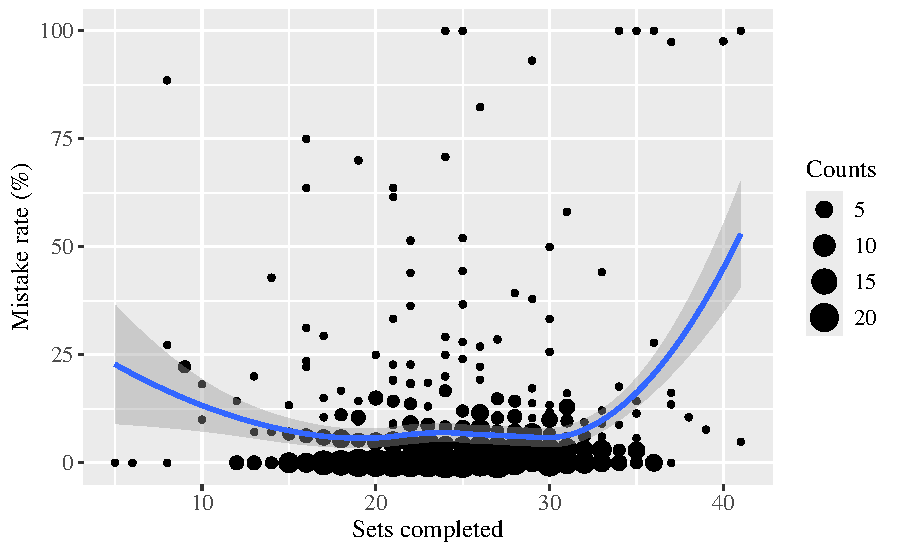
\includegraphics[width=0.75\linewidth]{output/figures/effort_tradeoffs_all.pdf}
\caption{All data}\label{fig-effort-tradeoffs-1}
\end{subfigure}
\begin{subfigure}{\linewidth}
\centering
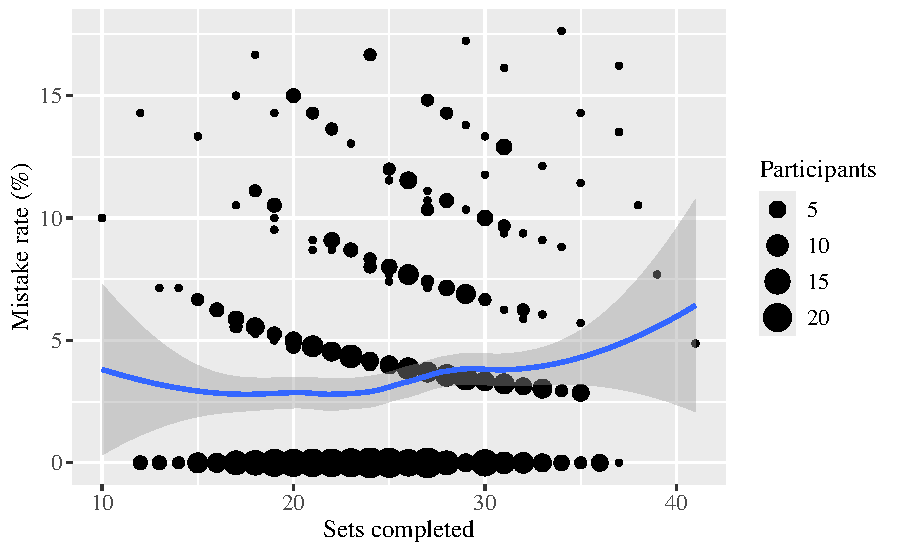
\includegraphics[width=0.75\linewidth]{output/figures/effort_tradeoffs_no_outliers.pdf}
\caption{Without outliers}\label{fig-effort-tradeoffs-2}
\end{subfigure}
\caption{Trade-offs between speed and accuracy in the slider task}\label{fig-effort-tradeoffs}
\end{figure}

\section{Results}\label{results}

\subsection{Econometric specifications}\label{econometric-specifications}

The main analysis of reference point effects on effort exertion and performance in the slider task uses regression (1), in which the saturated model to be estimated is
\[
log \frac {\mathbb{P}(Y_i = y_1)}{\mathbb{P}(Y_i = y_0)} = \beta_{1} + \beta_2 T_{2i} +\beta_3 T_{3i} +\beta_4 T_{4i} + \theta strict_i + \eta X_i + \varepsilon_i -(1)
\]
\(Y_i\) is the categorical variable for whether subject \(i\) achieved the targets, with four possible values: achieving both targets, achieving the speed target only, achieving the accuracy target only, and achieving none. Achieving none is set as the baseline (i.e.~\(y_0\)). Since no subject achieved the speed target (and by consequence both targets), there is only a single regression to run with \(y_1\) corresponding to achievement of the accuracy target. Note this is based on the \emph{recorded} mistake rate which depends on the assessment criteria as well. \(T_{ji}\) corresponds to subject \(i\) being in treatment group \(j\), with treatment 1 as the baseline (i.e.~omitted). \(strict_i\) is a dummy variable for whether the subject was assessed by the strict criterion. \(X_i\) is the vector of covariates and baseline metrics from the demo task. The estimated coefficients are readily interpretable as the increase in the log odds ratio of achieving the accuracy target relative to achieving no targets, or equivalently an increase in the odds ratio by the exponent \(e^{coefficient}\). This maps nicely into treatment effects on the probability of target achievement, which in turn measures the strength of reference point effects.

The KR model predicts that the magnitude of the treatment coefficients will be such that \(\beta_2 = \beta_4 < \beta_3\), whereas the appended model predicts \(\beta_2 > \beta_3\) and \(\beta_2 > \beta_4\), and in fact \(\beta_3\) and \(\beta_4\) may be insignificant. While I am testing for multiple treatment effects, I do not consider them under the same family of hypotheses, as the existence of probabilistic expectation effects (\(\beta_2 \text{ vs } \beta_3\)) should not affect that of cognitive complexity effects(\(\beta_2 \text{ vs } \beta_4\)), and both are prerequisited on the existence of reference points (\(\beta_2 \neq 0\)). In other words, they represent separate lines of inquiry which can stand on their own.

To complement the above analysis, I estimated regression (2) and (3) to examine treatment effects on mistake rate and sets completed respectively, which elucidate shifts in effort towards/ away from each dimension (intensive margin effects) even if they did not cause changes in target achievement (extensive margin effects.
\[
\begin{aligned}
& mistakerate_i = \gamma_1 + \gamma_2 T_{2i} + \gamma_3 T_{3i} + \gamma_4 T_{4i} + \phi strict_i + \psi X_i + \varepsilon_i -(2)
\\
& setscompleted_i = \delta_1 + \delta_2 T_{2i} + \delta_3 T_{3i} + \delta_4 T_{4i} + \mu strict_i + \nu X_i + \varepsilon_i -(3)
\end{aligned}
\]
The two models' predictions on the treatment coefficients remain the same as before. Note the predictions are now based on relative magnitudes and sign-agnostic; given the data, the direction of reference point effects will likely vary since accuracy performance in the control already exceeds the set target for the treated groups but the inverse holds for speed performance.

The above regression analysis was conducted for the pooled sample for increased power, as well as separately on the lab sample and combined class sample to check how effects may differ.

To further check experimental construct validity and that results are indeed stemming from reference point effects, I ran regression (4) on the pooled sample
\[
log \frac {\mathbb{P}(Y_i = y_1)}{\mathbb{P}(Y_i = y_0)} = \pi_1 + \pi_2 T_{2i} + \pi_3 T_{3i} + \pi_4 T_{4i} + \tau_1 \lambda_i + \tau_2(T_{2i}*\lambda_i) + \rho strict_i + \sigma X_i + \varepsilon_i -(4)
\]
\(\lambda_i\) is the subject's loss aversion level, measured in the manner of \textcite{campos-mercade.2024.gustibusdisputes}, with subjects having been asked to indicate the number of slider sets they are willing to complete under fixed and random piece rates. While those responses were not incentivised, they represent the best approximation given the budgetary constraints of the experiment. If treatment 2 effects are truly coming from the targets, they should increase in magnitude in the loss aversion level, so \(\tau_2\) should be in the same sign as \(\pi_2\). I focus on only treatment 2 for this verification since it is the most unambiguous on reference point effects with respect to the different models' predictions and to reduce the degrees of freedom exhausted. An analogue is estimated in regression (5) and (6) with \(mistakerate_i\) and \(setscompleted_i\) as the outcome variables respectively.

\subsection{Distributional comparisons of effort/ performance between treatments}\label{distributional-comparisons-of-effort-performance-between-treatments}

Prior to the regression analysis, I conducted non-parametric comparisons of sets completed and mistake rates in the slider task across treatment groups. Figure~\ref{fig-slider-performance-distribution-comparison} plots the cumulative distribution functions for the pooled sample. The distribution of sets completed is very similar across treatments with most subjects completing 25 sets and a rather symmetric spread around it. Mistake rates are also quite similar, though treatment 3 is dominated at low mistake rates up till 15\%. A joint Kruskal-Wallis test between treatments of differences in medians indeed finds no significant difference in sets completed (p-value = 0.11) but significant difference in the latter (p-value = 0.013, which is still significant under Bonferroni correction). Further pair-wise Kolmogorov distribution tests of differences in distributions reveal that the significant difference stems from treatment 3 (p-values = 0.0051 vs treatment 1, 0.049 vs treatment 2, and 0.012 vs treatment 4). This could indicate attenuation of reference point effects (if they exist), specifically in the accuracy dimension, from the increased conflict between the effort dimensions in treatment 3 where achieving both targets is more difficult.

Dissecting the sample into lab and class evinces that the differences found above arise from the class sample (Figure~\ref{fig-slider-performance-distribution-comparison-lab} and Figure~\ref{fig-slider-performance-distribution-comparison-class} in Appendix A1). Joint tests and pair-wise tests between treatments find no significant differences in sets completed nor mistake rates in the lab sample (the pair-wise test between treatments 2 and 4 does find significant difference in sets completed with p-value = 0.047, but the significance disappears after correction for multiple hypotheses testing). Conversely in the class sample, the joint test finds significant difference only for mistake rates and the pair-wise tests find the same but only for treatment 3 compared to other groups, paralleling the results in the pooled sample. In fact, this is likely stemming from the macroeconomics class sample; its treatment 3 has the highest mistake rate among all sub-sample-treatment combinations as seen previously. Thus, whatever implied effects are not robust across subsamples.

\begin{figure}[htbp]
\centering
\begin{subfigure}{\linewidth}
\centering
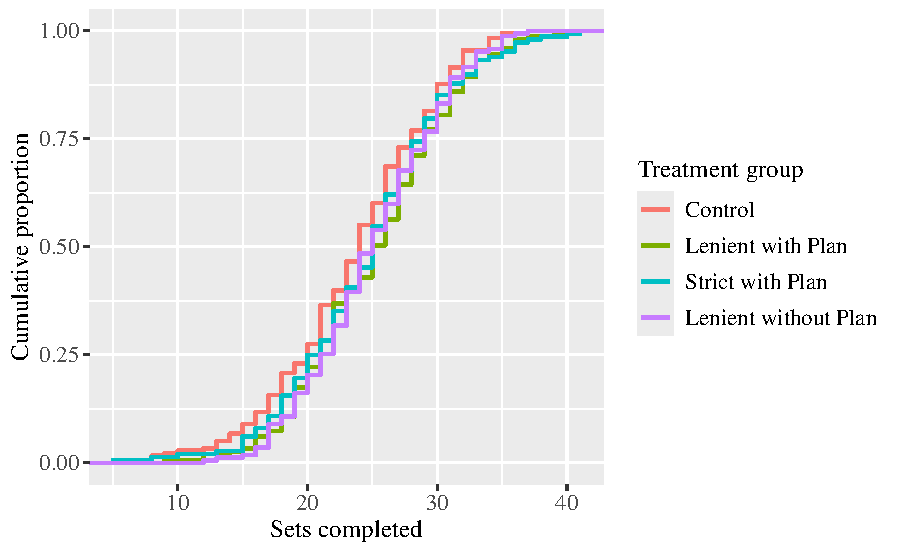
\includegraphics[width=0.75\linewidth]{output/figures/dist_comp_sets_completed_pooled.pdf}
\caption{Sets completed}\label{fig-slider-performance-distribution-comparison-1}
\end{subfigure}
\begin{subfigure}{\linewidth}
\centering
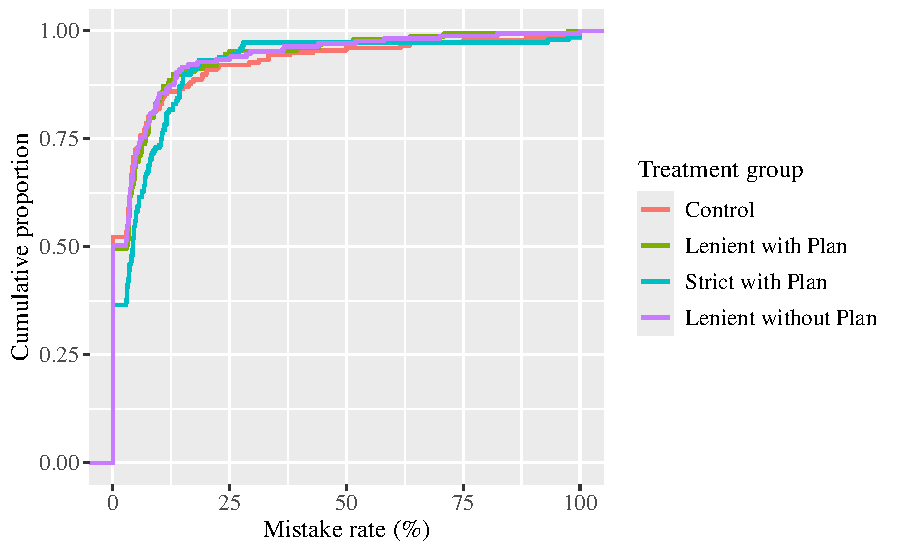
\includegraphics[width=0.75\linewidth]{output/figures/dist_comp_mistake_rate_pooled.pdf}
\caption{Mistake rate}\label{fig-slider-performance-distribution-comparison-2}
\end{subfigure}
\caption{Distributions of key performance metrics in the slider task across treatments (pooled sample)}\label{fig-slider-performance-distribution-comparison}
\end{figure}

\subsection{Regression estimates of treatment effects on effort}\label{regression-estimates-of-treatment-effects-on-effort}

Turning to a parametric estimation of treatment effects, regressions (1), (2), and (3) are estimated on the pooled sample and presented in Table~\ref{tbl-reg-target}, Table~\ref{tbl-reg-mistakes}, and Table~\ref{tbl-reg-sets} respectively (full regression estimates in Appendix A1). For each regression, model (1) regresses the outcome on the treatments alone; model (2) controls for covariates; model (3) controls for baseline performance in the demo task; and model (4) controls for both. We see that the treatment coefficient estimates do exhibit considerable variation in their magnitudes across the different models in all regressions. Since there were some covariate imbalance between treatments found in the sample, the estimates from the most basic model (1) are likely least reliable. I focus on estimates from models (3) and (4), which have the lowest Bayesian Information Criterion and Akaike Information Criterion measures respectively in regression (1) and the highest adjusted \(R^2\) values in regressions (2) and (3) \footnote{The BIC more heavily penalises additional model parameters and hence rates model (4) worse despite it fitting the data better. The BIC is consistent in selecting the ``true'' model i.e.~it selects the true model as sample size approaches infinity, so it is appropriate for large sample sizes, though it is uncertain how well that holds here. Model (4) also suffers in regression (2) due to the high skewness of the outcome toward zero and high dimensionality of the regressors, causing problems with standard error computations.}. Note model (3) also has the second lowest AIC in regression (1) and much higher adjusted \(R^2\) values than model (2), meaning that the baseline performance metrics do a relatively good job of predicting task effort and performance, capturing most of the covariate effects and beyond.

Strikingly, regardless of the model used, all treatment effects on the likelihood of achieving the accuracy target are negative, though not significant, which seems to pose a paradox to hypothesized reference point effects. However, note treatment effects on sets completed are positive and significant at 5\% across the board. This is consistent with the existence of reference point effects and subjects' inherent prioritisation of accuracy (relative to the set targets). Consider that subjects already had internally conceived targets for speed and accuracy, which were mostly below 45 sets completed and below 10\% mistake rate respectively; this is congruent with the mean performance metrics in the control. Thus, externally setting targets of 45 sets completed and 10\% mistake rate shifted subjects' focus away from their internal targets to the external ones, inducing greater effort in the speed dimension at the expense of the effort in the accuracy dimension. This would produce the effects observed in regressions (1) and (2). The insignificant results for the former likely reflects that subjects still valued performance in accuracy much more than speed and hence were unlikely to stray from the accuracy target. This is corroborated by available survey responses to the question of why the subject did not attempt to achieve both targets, with most citing that they focused on accuracy more. A caveat is that treatment effects on mistake rate are all negative also (i.e positive effect on accuracy), which could reflect different effects at the extensive and intensive margins, but are also less credible given the poorer data fit.

In this same vein of reasoning, now restricting focus to models (3) and (4), we see that treatment 3 does show weaker reference point effects than treatment 2, with smaller coefficient magnitudes in all regressions. However, the difference in coefficients are not significant: comparing effects on the likelihood of achieving the accuracy target, p-value = 0.38 for model (3) and 0.88 for model (4); comparing effects on mistake rate, p-value = 0.64 for model (3) and unestimable for model (4); comparing effects on sets completed, p-value = 0.34 for model (3) and 0.28 for model (4). This can be attributed to a small base effect of the reference points, with treatment 2 only increasing sets completed by 1.24 on average relative to the mean of \ControlMeanSets{} in the control, and decreasing the odds of achieving the accuracy target by 0.58 times as opposed to the control increasing the odds by 10.59 times (based on model 4 estimates). Thus, any attenuation effects would be even smaller (weakly) and harder to detect.

Conversely, treatment 4 does not show weaker reference point effects; the magnitudes are smaller in regression (1) but larger in (2) and (3). A considerable portion of respondents (107 out of 285) said that the explanation of the targets did not make it easier for them to achieve both targets nor make them more motivated to do so, so the treatments may not have worked as intended. The mean time spent on instructions for treatments 2 and 3 (59.34 and 52.32 seconds respectively) is much lower than that for treatment 4 (143.30 seconds), suggesting that subjects may not have actually digested the explanation of the targets in the former.

There are also some statistically significant covariate effects on effort and performance \footnote{Covariate effects on mistake rates are not analysed since the saturated model is unstable and the model with only covariates has very poor fit.}. Those who studied undergraduate economics are 2.44 times more likely to achieve the accuracy target, though this could also be interpreted as class sample effects. Those working in professional services are 8.94 times more likely to achieve the accuracy target, but complete 1.5 sets less on average. Surprisingly, using a mouse has no effect on achievement of the accuracy target, likely because subjects' focus on this aspect more than compensate for mouse usage, but does increase sets completed by 1 on average. Female subjects complete 1 less set on average and Black subjects complete 1.5 sets less on average. Some significant effects for income brackets are observed but there are no meaningful patterns. Having an education level of below a high school diploma critically reduces sets completed by 3 but it is likely due to pure chance given there is only one observation in this category.

The treatment effects found above are somewhat robust to estimation by subsamples (tables in Appendix A1). The reference point effects in treatment 2 stay similar in the lab and class samples, with negative effects on likelihood of achieving the accuracy target and positive effects on sets completed, although the latter are no longer significant, likely due to smaller sample size and noisier estimates (much larger standard deviations). The effect sizes of treatment 4 relative to treatment 2 remain ambiguous in both subsamples. Treatment 3 effects for the lab sample are congruent with the pooled sample, being less negative for accuracy target achievements and less positive for sets completed relative to treatment 2, with significant differences found for the former (p-values = 0.024 for model (3) and 0.038 for model (4)). The main difference lies in treatment 3 effects for class sample, which show more negative effects for accuracy target achievement, though they are still less positive for sets completed; no differences are significant. The discrepancy is plausibly attributed to sampling error in the macroeconomic class sample whose treatment 3 had the highest mistake rate.

\begin{table}
\centering
% Generated by the R scripts in code/; the note is set at the width of the table
\ifdefined\regtablebox\else\newsavebox{\regtablebox}\fi
\sbox{\regtablebox}{%
\begin{tabular}{l c c c c}
\toprule
 & \multicolumn{4}{c}{Log odds of meeting the accuracy target} \\
\cmidrule(lr){2-5}
 & (1) & (2) & (3) & (4) \\
\midrule
Lenient with Plan    & $-0.53$      & $-0.35$      & $-0.76^{*}$  & $-0.54$     \\
                     & $(0.38)$     & $(0.44)$     & $(0.40)$     & $(0.46)$    \\
Strict with Plan     & $-0.52^{*}$  & $-0.57^{*}$  & $-0.42$      & $-0.47$     \\
                     & $(0.29)$     & $(0.33)$     & $(0.32)$     & $(0.37)$    \\
Lenient without Plan & $-0.03$      & $-0.12$      & $-0.08$      & $-0.08$     \\
                     & $(0.43)$     & $(0.47)$     & $(0.46)$     & $(0.51)$    \\
Constant             & $3.41^{***}$ & $3.00^{***}$ & $3.29^{***}$ & $2.36^{**}$ \\
                     & $(0.43)$     & $(0.76)$     & $(0.68)$     & $(0.99)$    \\
\midrule
Baselines            & No           & No           & Yes          & Yes         \\
Covariates           & No           & Yes          & No           & Yes         \\
Observations            & $642$        & $549$        & $642$        & $549$       \\
\bottomrule
\end{tabular}
}%
\begin{minipage}{\wd\regtablebox}
\usebox{\regtablebox}

\smallskip
{\footnotesize\raggedright\textit{Notes:} Logit estimates, with standard errors in parentheses. The outcome is meeting the accuracy target, that is, a recorded mistake rate of at most 10\%. The omitted group is Control. All specifications control for whether the strict criterion was applied. Baselines are sets attempted, sets completed and mistakes in the demo task; covariates are gender, race, household income, education, economics studies, occupation and mouse use. Specifications with covariates use the participants who answered all covariate questions. $^{***}p<0.01$, $^{**}p<0.05$, $^{*}p<0.1$.\par}
\end{minipage}

\caption{Treatment effects on accuracy target achivement likelihood (pooled sample)}\label{tbl-reg-target}
\end{table}

\begin{table}
\centering
% Generated by the R scripts in code/
\begin{tabular}{l c c c c}
\toprule
 & \multicolumn{4}{c}{Mistake rate (\%)} \\
\cmidrule(lr){2-5}
 & (1) & (2) & (3) & (4) \\
\midrule
Lenient with Plan    & $-2.22$  & $-3.53^{*}$ & $-1.75$  & $-3.56^{**}$ \\
                     & $(1.91)$ & $(1.95)$    & $(1.66)$ & $(1.71)$     \\
Strict with Plan     & $0.30$   & $-0.06$     & $-1.07$  & $-1.62$      \\
                     & $(1.91)$ & $(2.01)$    & $(1.53)$ & $(1.68)$     \\
Lenient without Plan & $-2.37$  & $-2.96$     & $-2.20$  & $-3.06$      \\
                     & $(1.95)$ & $(2.13)$    & $(1.75)$ & $(1.96)$     \\
\midrule
Baselines            & No       & No          & Yes      & Yes          \\
Covariates           & No       & Yes         & No       & Yes          \\
Observations            & $642$    & $547$       & $642$    & $547$        \\
\bottomrule
\end{tabular}

\caption{Treatment effects on mistake rate (pooled sample)}\label{tbl-reg-mistakes}
\end{table}

\begin{table}
\centering

\begin{tabular}{l c c c c}
\hline
 & \multicolumn{4}{c}{Sets completed} \\
\cline{2-5}
 & Model 1 & Model 2 & Model 3 & Model 4 \\
\hline
(Intercept) & $23.52^{***}$ & $22.60^{***}$ & $8.41^{***}$ & $8.89^{***}$ \\
            & $(0.79)$      & $(1.23)$      & $(0.97)$     & $(1.28)$     \\
treatment2  & $1.69^{*}$    & $1.60^{*}$    & $1.46^{*}$   & $1.24^{*}$   \\
            & $(0.81)$      & $(0.77)$      & $(0.57)$     & $(0.59)$     \\
treatment3  & $1.15$        & $0.74$        & $0.95$       & $0.66$       \\
            & $(0.69)$      & $(0.68)$      & $(0.49)$     & $(0.52)$     \\
treatment4  & $1.53$        & $1.36$        & $1.59^{**}$  & $1.36^{*}$   \\
            & $(0.80)$      & $(0.76)$      & $(0.61)$     & $(0.63)$     \\
\hline
Baselines   & No            & No            & Yes          & Yes          \\
Covariates  & No            & Yes           & No           & Yes          \\
\hline
R$^2$       & $0.01$        & $0.22$        & $0.46$       & $0.53$       \\
Adj. R$^2$  & $0.01$        & $0.18$        & $0.45$       & $0.50$       \\
Num. obs.   & $642$         & $549$         & $642$        & $549$        \\
RMSE        & $5.78$        & $5.30$        & $4.29$       & $4.13$       \\
\hline
\multicolumn{5}{l}{\scriptsize{$^{***}p<0.001$; $^{**}p<0.01$; $^{*}p<0.05$}}
\end{tabular}


\caption{Treatment effects on sets completed (pooled sample)}\label{tbl-reg-sets}
\end{table}

\subsection{Verification of reference point effects}\label{verification-of-reference-point-effects}

A final robustness check of the purported reference point effects is done by interacting treatment effects with loss aversion levels in the pooled sample.

Loss aversion levels were estimated following \textcite{campos-mercade.2024.gustibusdisputes} which assume KR reference-dependent preferences. In the post-task survey, subjects were asked to indicate the number of correctly completed sets they were willing to do under different payment structures, which consisted of seven different fixed piece rates and seven different random piece rates. The random piece rate paid out either a high piece rate or low piece rate with equal probabilities, and each had an expected payment equal to one of the fixed piece rates. Assuming an effort cost function of \(c(e) = \frac {1}{\alpha + \omega} e^\omega\) as in the original paper and based upon \textcite{augenblick.2019.experimenttime}, we obtain the reduced form approximation
\[
\begin{aligned}
& log(e_i) \approx J_i + K_i log(\bar{w}) - L_i \frac{\Delta w}{\bar w} \\
& \text{Where} \\
& J_i = \frac {log(\alpha_i)}{\omega_i - 1}; \space K_i = \frac {1}{\omega_i - 1}; \space L_i = \frac {\lambda_i -1}{4(\omega_i - 1)} = \frac {1}{4} K_i (\lambda_i -1)
\end{aligned}
\]
\(\bar w\) is the average piece rate, which is just equal to the piece rate for fixed payments, whereas \(\Delta w = w_h - w_l\) is the piece rate spread where \(w_h\) is the high piece rate and \(w_l\) is the low piece rate paid out in random payments, and equal to zero for fixed payments. Recall that \(\lambda_i\) is the loss aversion parameter, so \(L_i\) acts as its reduced form estimate. Given the approximation holds with some mean zero error term, we can estimate the equation using OLS regression.\footnote{Estimates of \(\lambda_i\) had to be top-coded at 4.33 given the maximum \(\frac{\Delta w}{\bar w} = 1.2\) in the survey, otherwise the logarithms in the approximated equation below will be undefined.
  \[
  log(e_i) = J_i + K_i log(\bar{w}) + K_i log(1 + 0.25 (1 - \lambda_i) \frac{\Delta w}{\bar w})
  \]
  Estimates were also bottom-coded at 0 as negative values are difficult to interpret (would imply utility gains from losses).}

After obtaining structural estimates of the loss aversion parameters, I run regressions (4), (5) and (6) using just models (3) and (4) now, omitting The results in Table~\ref{tbl-reg-target-la}, Table~\ref{tbl-reg-mistakes-la}, and Table~\ref{tbl-reg-sets-la} detract from the reference point effects posited above as the coefficient on the interaction term between treatment 2 and the loss aversion level is positive when the outcome is the log odds of accuracy target achievement and negative when the outcome is sets completed, which contradicts the hypothesis that more loss averse individuals should be more affected by the set targets to induce greater effort in speed and less in accuracy.

A caveat is that the loss aversion estimation could be unreliable since it was unincentivised and hence the reports are likely to suffer from hypothetical bias. Almost half of the raw estimates (248 out of 503) lie beyond the upper and lower bounds allowed by the estimation, with a considerable portion (176) having negative loss aversion parameters before top and bottom-coding adjustments. Data quality aside, the interaction between loss aversion and treatment effects is also ambiguous, since loss aversion can be with respect to both internally conceived targets and externally set ones, hence it could either counteract or reinforce the suggested reference point effects. These complications in interpretation arise due to the different directions of effect exerted by the reference points in each effort/ performance dimension.

Nevertheless, in accordance with the original analysis plan and hypothesis, this exercise refutes that treatment effects can be attributed to reference points, hence the (in)validation of both models' predictions are inconclusive. Since treatment effects are dubious and not significant, this was a moot point, I do not proceed with heterogeneity analysis.

\begin{table}
\centering
% Generated by the R scripts in code/; the note is set at the width of the table
\ifdefined\regtablebox\else\newsavebox{\regtablebox}\fi
\sbox{\regtablebox}{%
\begin{tabular}{l c c}
\toprule
 & \multicolumn{2}{c}{Log odds of meeting the accuracy target} \\
\cmidrule(lr){2-3}
 & (1) & (2) \\
\midrule
Lenient with Plan                        & $-1.09^{*}$   & $-1.25^{*}$   \\
                                         & $(0.59)$      & $(0.68)$      \\
Strict with Plan                         & $-0.33$       & $-0.39$       \\
                                         & $(0.38)$      & $(0.43)$      \\
Lenient without Plan                     & $-0.37$       & $-0.29$       \\
                                         & $(0.52)$      & $(0.57)$      \\
Strict criterion                         & $-2.35^{***}$ & $-2.61^{***}$ \\
                                         & $(0.52)$      & $(0.59)$      \\
Loss aversion ($\lambda_i$)              & $-0.11$       & $-0.13$       \\
                                         & $(0.10)$      & $(0.12)$      \\
Lenient with Plan $\times$ loss aversion & $0.36$        & $0.42$        \\
                                         & $(0.28)$      & $(0.30)$      \\
Constant                                 & $3.88^{***}$  & $3.12^{**}$   \\
                                         & $(0.84)$      & $(1.21)$      \\
\midrule
Baselines                                & Yes           & Yes           \\
Covariates                               & No            & Yes           \\
Observations                                & $503$         & $460$         \\
\bottomrule
\end{tabular}
}%
\begin{minipage}{\wd\regtablebox}
\usebox{\regtablebox}

\smallskip
{\footnotesize\raggedright\textit{Notes:} Logit estimates, with standard errors in parentheses. The outcome is meeting the accuracy target, that is, a recorded mistake rate of at most 10\%. The omitted group is Control. Loss aversion is the participant's estimated $\lambda_i$, top-coded at 4.33 and bottom-coded at 0. Both specifications control for baseline performance in the demo task (sets attempted, sets completed and mistakes); column (2) also controls for gender, race, household income, education, economics studies, occupation and mouse use. The sample is the participants whose loss aversion could be estimated and, in column (2), who answered all covariate questions. $^{***}p<0.01$, $^{**}p<0.05$, $^{*}p<0.1$.\par}
\end{minipage}

\caption{Treatment effects on target achievement interacted with loss aversion}\label{tbl-reg-target-la}
\end{table}

\begin{table}
\centering
% Generated by the R scripts in code/; the note is set at the width of the table
\ifdefined\regtablebox\else\newsavebox{\regtablebox}\fi
\sbox{\regtablebox}{%
\begin{tabular}{l c c}
\toprule
 & \multicolumn{2}{c}{Mistake rate (\%)} \\
\cmidrule(lr){2-3}
 & (1) & (2) \\
\midrule
Lenient with Plan                        & $-2.51$     & $-1.83$     \\
                                         & $(1.95)$    & $(2.02)$    \\
Strict with Plan                         & $-1.11$     & $-1.02$     \\
                                         & $(1.61)$    & $(1.68)$    \\
Lenient without Plan                     & $-1.84$     & $-1.40$     \\
                                         & $(2.00)$    & $(2.17)$    \\
Strict criterion                         & $-2.28^{*}$ & $-1.45$     \\
                                         & $(1.35)$    & $(1.21)$    \\
Loss aversion                            & $-0.00$     & $-0.05$     \\
                                         & $(0.52)$    & $(0.58)$    \\
Lenient with Plan $\times$ Loss aversion & $-0.71$     & $-1.07$     \\
                                         & $(0.76)$    & $(0.82)$    \\
Constant                                 & $6.68^{**}$ & $9.04^{**}$ \\
                                         & $(2.75)$    & $(4.38)$    \\
\midrule
Baselines                                & Yes         & Yes         \\
Covariates                               & No          & Yes         \\
Observations                                & $503$       & $453$       \\
\bottomrule
\end{tabular}
}%
\begin{minipage}{\wd\regtablebox}
\usebox{\regtablebox}

\smallskip
{\footnotesize\raggedright\textit{Notes:} OLS estimates, with heteroskedasticity-robust (HC3) standard errors in parentheses. The omitted group is Control. Loss aversion is the participant's estimated $\lambda_i$, top-coded at 4.33 and bottom-coded at 0. Both specifications control for baseline performance in the demo task (sets attempted, sets completed and mistakes); column (2) also controls for gender, race, household income, education level, economics studies, occupation and mouse use. The sample is the participants whose loss aversion could be estimated and, in column (2), who answered all covariate questions, except the few non-binary participants. $^{***}p<0.01$, $^{**}p<0.05$, $^{*}p<0.1$.\par}
\end{minipage}

\caption{Treatment effects on mistake rate interacted with loss aversion}\label{tbl-reg-mistakes-la}
\end{table}

\begin{table}
\centering
% Generated by the R scripts in code/
\begin{tabular}{l c c}
\toprule
 & \multicolumn{2}{c}{Sets completed} \\
\cmidrule(lr){2-3}
 & (1) & (2) \\
\midrule
Lenient with Plan                        & $1.28$       & $1.00$       \\
                                         & $(0.79)$     & $(0.86)$     \\
Strict with Plan                         & $0.71$       & $0.53$       \\
                                         & $(0.56)$     & $(0.63)$     \\
Lenient without Plan                     & $1.45^{**}$  & $1.38^{*}$   \\
                                         & $(0.71)$     & $(0.72)$     \\
Strict criterion                         & $0.15$       & $0.28$       \\
                                         & $(0.54)$     & $(0.55)$     \\
Loss aversion                            & $0.11$       & $0.06$       \\
                                         & $(0.14)$     & $(0.14)$     \\
Lenient with Plan $\times$ Loss aversion & $-0.05$      & $-0.03$      \\
                                         & $(0.26)$     & $(0.27)$     \\
Constant                                 & $8.21^{***}$ & $8.22^{***}$ \\
                                         & $(1.13)$     & $(1.29)$     \\
\midrule
Baselines                                & Yes          & Yes          \\
Covariates                               & No           & Yes          \\
Observations                                & $503$        & $457$        \\
\bottomrule
\end{tabular}

\caption{Treatment effects on sets completed interacted with loss aversion}\label{tbl-reg-sets-la}
\end{table}

\newpage

\section{Conclusion}\label{conclusion}

This paper has investigated potential interaction effects between multi-dimensional reference points, specifically the attenuation of conflicting reference points due to low probabilistic expectations of concurrently achieving them and/ or cognitive complexity in reconciling them. The experiment found some weak evidence for such effects, but they were mostly statistically insignificant and not robust to sampling differences. They also failed the construct validity check of whether the effects are indeed stemming from reference points (though the verification method itself was problematic due to unincentivised responses).

Overall, budgetary and time constraints led to less than ideal experimental design which failed to offer conclusive insights on how humans aggregate across reference points in multiple dimensions, with neither strong support for the original or augmented KR model. However, the experimental results do highlight the dynamics between internally conceived and externally imposed targets in reference point formation, which signals a potential new avenue for research.

\newpage

\section{Bibliography}\label{bibliography}

\printbibliography[heading=none]

\newpage

\section{Appendix}\label{appendix}

\subsection{A1. Figures and tables}\label{a1.-figures-and-tables}

\begin{figure}[H]
\centering
\begin{subfigure}{\linewidth}
\centering
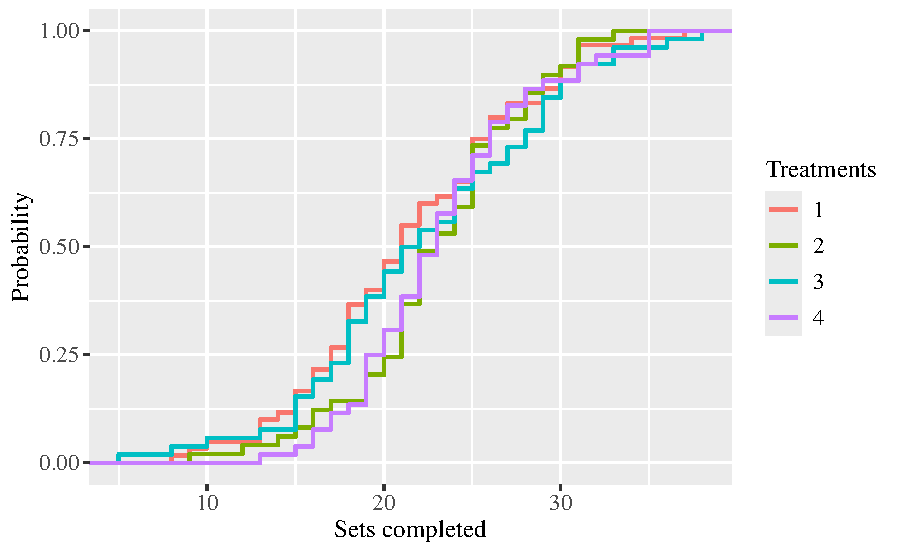
\includegraphics[width=0.75\linewidth]{output/figures/dist_comp_sets_completed_lab.pdf}
\caption{Sets completed}\label{fig-slider-performance-distribution-comparison-lab-1}
\end{subfigure}
\begin{subfigure}{\linewidth}
\centering
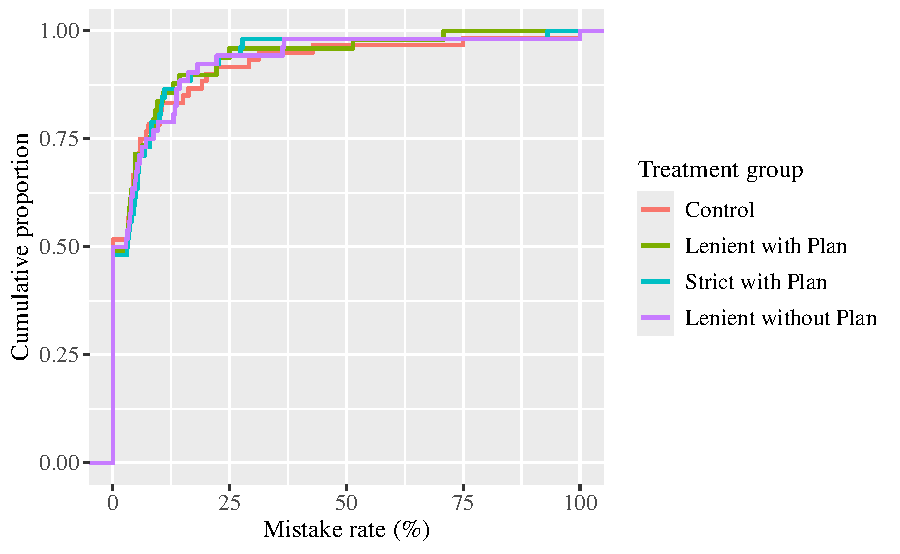
\includegraphics[width=0.75\linewidth]{output/figures/dist_comp_mistake_rate_lab.pdf}
\caption{Mistake rate}\label{fig-slider-performance-distribution-comparison-lab-2}
\end{subfigure}
\caption{Distributions of key performance metrics in the slider task across treatments (lab sample)}\label{fig-slider-performance-distribution-comparison-lab}
\end{figure}

\begin{figure}[htbp]
\centering
\begin{subfigure}{\linewidth}
\centering
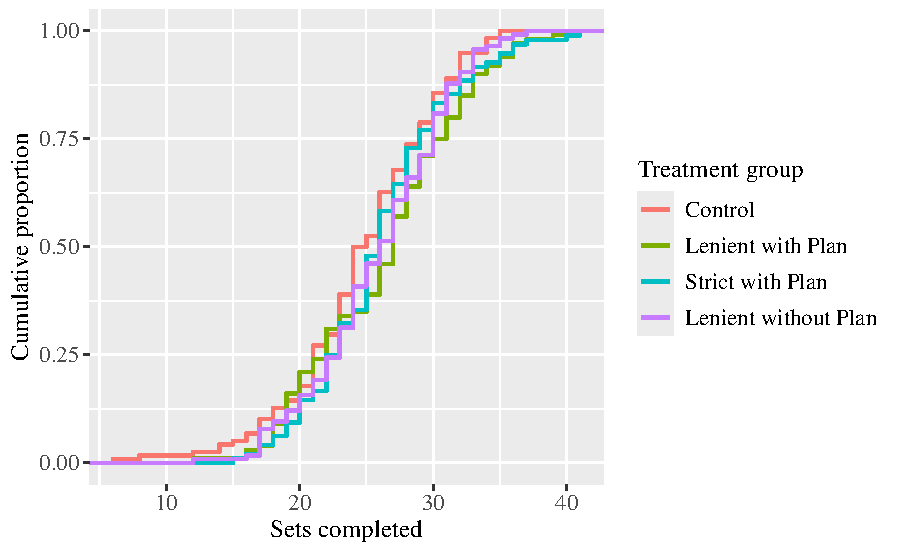
\includegraphics[width=0.75\linewidth]{output/figures/dist_comp_sets_completed_class.pdf}
\caption{Sets completed}\label{fig-slider-performance-distribution-comparison-class-1}
\end{subfigure}
\begin{subfigure}{\linewidth}
\centering
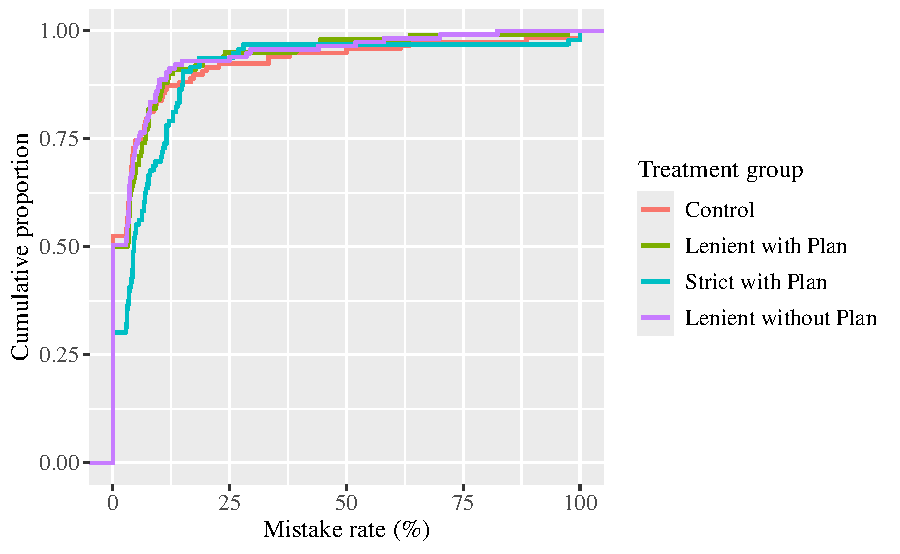
\includegraphics[width=0.75\linewidth]{output/figures/dist_comp_mistake_rate_class.pdf}
\caption{Mistake rate}\label{fig-slider-performance-distribution-comparison-class-2}
\end{subfigure}
\caption{Distributions of key performance metrics in the slider task across treatments (class sample)}\label{fig-slider-performance-distribution-comparison-class}
\end{figure}

\begin{table}[p]
\centering
{\scriptsize\renewcommand{\arraystretch}{0.85}

\begin{tabular}{l c c c c}
\hline
 & \multicolumn{4}{c}{Log odds of achieving accuracy target} \\
\cline{2-5}
 & Model 1 & Model 2 & Model 3 & Model 4 \\
\hline
(Intercept)                     & $3.41^{***}$  & $3.00^{***}$  & $3.29^{***}$  & $2.36^{*}$    \\
                                & $(0.43)$      & $(0.76)$      & $(0.68)$      & $(0.99)$      \\
treatment2                      & $-0.53$       & $-0.35$       & $-0.76$       & $-0.54$       \\
                                & $(0.38)$      & $(0.44)$      & $(0.40)$      & $(0.46)$      \\
treatment3                      & $-0.52$       & $-0.57$       & $-0.42$       & $-0.47$       \\
                                & $(0.29)$      & $(0.33)$      & $(0.32)$      & $(0.37)$      \\
treatment4                      & $-0.03$       & $-0.12$       & $-0.08$       & $-0.08$       \\
                                & $(0.43)$      & $(0.47)$      & $(0.46)$      & $(0.51)$      \\
criterionstrict                 & $-1.81^{***}$ & $-1.97^{***}$ & $-2.22^{***}$ & $-2.31^{***}$ \\
                                & $(0.38)$      & $(0.44)$      & $(0.42)$      & $(0.48)$      \\
genderFemale                    &               & $0.07$        &               & $0.04$        \\
                                &               & $(0.29)$      &               & $(0.31)$      \\
genderNon-binary                &               & $16.05$       &               & $15.37$       \\
                                &               & $(1329.79)$   &               & $(1341.41)$   \\
raceAsian                       &               & $0.36$        &               & $0.21$        \\
                                &               & $(0.32)$      &               & $(0.34)$      \\
raceBlack                       &               & $0.31$        &               & $0.21$        \\
                                &               & $(0.51)$      &               & $(0.55)$      \\
raceHispanic                    &               & $1.05$        &               & $0.89$        \\
                                &               & $(0.60)$      &               & $(0.62)$      \\
raceMixed                       &               & $-0.50$       &               & $-0.22$       \\
                                &               & $(0.58)$      &               & $(0.72)$      \\
income25,000 - 49,999           &               & $-0.18$       &               & $-0.39$       \\
                                &               & $(0.70)$      &               & $(0.73)$      \\
income50,000 - 74,999           &               & $-0.68$       &               & $-0.59$       \\
                                &               & $(0.65)$      &               & $(0.70)$      \\
income75,000 - 119,999          &               & $-1.09$       &               & $-1.26^{*}$   \\
                                &               & $(0.59)$      &               & $(0.64)$      \\
income120,000 - 199,999         &               & $0.44$        &               & $0.20$        \\
                                &               & $(0.69)$      &               & $(0.73)$      \\
income200,000 and over          &               & $-0.70$       &               & $-0.66$       \\
                                &               & $(0.54)$      &               & $(0.58)$      \\
eduBelow high school diploma    &               & $16.37$       &               & $17.18$       \\
                                &               & $(3956.18)$   &               & $(3956.18)$   \\
eduHigh school diploma          &               & $0.44$        &               & $0.64$        \\
                                &               & $(0.61)$      &               & $(0.67)$      \\
econYes                         &               & $0.78$        &               & $0.89^{*}$    \\
                                &               & $(0.43)$      &               & $(0.46)$      \\
occupationAcademia              &               & $0.21$        &               & $0.27$        \\
                                &               & $(0.74)$      &               & $(0.77)$      \\
occupationClerical              &               & $1.09$        &               & $2.17$        \\
                                &               & $(1.16)$      &               & $(1.58)$      \\
occupationHigh-tech mfg or eng  &               & $-0.55$       &               & $-0.45$       \\
                                &               & $(0.90)$      &               & $(0.93)$      \\
occupationManagerial            &               & $-0.29$       &               & $0.41$        \\
                                &               & $(0.85)$      &               & $(0.91)$      \\
occupationProfessional services &               & $1.57$        &               & $2.19^{*}$    \\
                                &               & $(0.81)$      &               & $(0.89)$      \\
occupationUnemployed            &               & $16.28$       &               & $16.77$       \\
                                &               & $(1117.14)$   &               & $(1059.22)$   \\
occupationOther                 &               & $-1.76$       &               & $-2.16^{*}$   \\
                                &               & $(1.02)$      &               & $(1.06)$      \\
mouseYes                        &               & $0.20$        &               & $-0.01$       \\
                                &               & $(0.29)$      &               & $(0.31)$      \\
demo\_sets\_attempted           &               &               & $0.49^{***}$  & $0.47^{**}$   \\
                                &               &               & $(0.14)$      & $(0.17)$      \\
demo\_sets\_completed           &               &               & $-0.28^{*}$   & $-0.15$       \\
                                &               &               & $(0.13)$      & $(0.15)$      \\
demo\_mistakes                  &               &               & $-0.61^{***}$ & $-0.63^{***}$ \\
                                &               &               & $(0.09)$      & $(0.11)$      \\
\hline
AIC                             & $474.96$      & $420.88$      & $419.62$      & $381.34$      \\
BIC                             & $497.28$      & $537.20$      & $455.34$      & $510.59$      \\
Log Likelihood                  & $-232.48$     & $-183.44$     & $-201.81$     & $-160.67$     \\
Num. obs.                       & $642$         & $549$         & $642$         & $549$         \\
\hline
\multicolumn{5}{l}{\scriptsize{$^{***}p<0.001$; $^{**}p<0.01$; $^{*}p<0.05$}}
\end{tabular}

\par}
\caption{Treatment effects on accuracy target achievement likelihood (pooled sample)}\label{tbl-reg-target-full}
\end{table}

\begin{table}[p]
\centering
{\scriptsize\renewcommand{\arraystretch}{0.85}
% Generated by the R scripts in code/
\begin{tabular}{l c c c c}
\toprule
 & \multicolumn{4}{c}{Mistake rate (\%)} \\
\cmidrule(lr){2-5}
 & (1) & (2) & (3) & (4) \\
\midrule
Lenient with Plan        & $-2.22$      & $-3.53^{*}$   & $-1.75$      & $-3.56^{**}$  \\
                         & $(1.91)$     & $(1.95)$      & $(1.66)$     & $(1.71)$      \\
Strict with Plan         & $0.30$       & $-0.06$       & $-1.07$      & $-1.62$       \\
                         & $(1.91)$     & $(2.01)$      & $(1.53)$     & $(1.68)$      \\
Lenient without Plan     & $-2.37$      & $-2.96$       & $-2.20$      & $-3.06$       \\
                         & $(1.95)$     & $(2.13)$      & $(1.75)$     & $(1.96)$      \\
Strict criterion         & $-1.22$      & $-1.93$       & $-1.11$      & $-2.24^{*}$   \\
                         & $(1.45)$     & $(1.45)$      & $(1.27)$     & $(1.28)$      \\
Baseline sets attempted  &              &               & $-3.61$      & $-3.31$       \\
                         &              &               & $(2.40)$     & $(2.45)$      \\
Baseline sets completed  &              &               & $3.20$       & $3.08$        \\
                         &              &               & $(2.42)$     & $(2.46)$      \\
Baseline mistakes        &              &               & $5.64^{***}$ & $5.58^{***}$  \\
                         &              &               & $(1.08)$     & $(1.21)$      \\
Female                   &              & $0.69$        &              & $1.63$        \\
                         &              & $(1.31)$      &              & $(1.28)$      \\
Race                     &              &               &              &               \\
\quad Asian              &              & $-3.09^{**}$  &              & $-2.37^{*}$   \\
                         &              & $(1.48)$      &              & $(1.35)$      \\
\quad Black              &              & $-4.87^{***}$ &              & $-2.96^{*}$   \\
                         &              & $(1.72)$      &              & $(1.51)$      \\
\quad Hispanic           &              & $-4.07^{*}$   &              & $-2.18$       \\
                         &              & $(2.10)$      &              & $(2.04)$      \\
\quad Other              &              & $4.79$        &              & $0.04$        \\
                         &              & $(5.54)$      &              & $(4.26)$      \\
Household income         &              &               &              &               \\
\quad \$25,000--49,999   &              & $-0.25$       &              & $-0.70$       \\
                         &              & $(2.27)$      &              & $(2.21)$      \\
\quad \$50,000--74,999   &              & $3.46$        &              & $1.18$        \\
                         &              & $(3.27)$      &              & $(2.79)$      \\
\quad \$75,000--119,999  &              & $5.57^{*}$    &              & $4.05$        \\
                         &              & $(3.06)$      &              & $(2.55)$      \\
\quad \$120,000--199,999 &              & $-3.28^{*}$   &              & $-3.09^{*}$   \\
                         &              & $(1.81)$      &              & $(1.76)$      \\
\quad \$200,000 and over &              & $1.34$        &              & $-0.86$       \\
                         &              & $(2.14)$      &              & $(2.01)$      \\
No college               &              & $0.23$        &              & $-0.24$       \\
                         &              & $(2.97)$      &              & $(2.79)$      \\
Studied economics        &              & $-1.26$       &              & $-1.44$       \\
                         &              & $(1.70)$      &              & $(1.62)$      \\
Student                  &              & $0.87$        &              & $0.94$        \\
                         &              & $(1.72)$      &              & $(1.76)$      \\
Used mouse               &              & $-2.79^{**}$  &              & $-1.56$       \\
                         &              & $(1.28)$      &              & $(1.16)$      \\
Constant                 & $8.96^{***}$ & $11.68^{***}$ & $7.66^{***}$ & $10.27^{***}$ \\
                         & $(1.98)$     & $(3.25)$      & $(2.73)$     & $(3.61)$      \\
\midrule
Observations                & $642$        & $547$         & $642$        & $547$         \\
\bottomrule
\end{tabular}
\par}
\caption{Treatment effects on mistakes rate (pooled sample)}\label{tbl-reg-mistakes-full}
\end{table}

\begin{table}[p]
\centering
{\scriptsize\renewcommand{\arraystretch}{0.85}

\begin{tabular}{l c c c c}
\hline
 & \multicolumn{4}{c}{Sets completed} \\
\cline{2-5}
 & Model 1 & Model 2 & Model 3 & Model 4 \\
\hline
(Intercept)                     & $23.52^{***}$ & $22.60^{***}$ & $8.41^{***}$ & $8.89^{***}$  \\
                                & $(0.79)$      & $(1.23)$      & $(0.97)$     & $(1.28)$      \\
treatment2                      & $1.69^{*}$    & $1.60^{*}$    & $1.46^{*}$   & $1.24^{*}$    \\
                                & $(0.81)$      & $(0.77)$      & $(0.57)$     & $(0.59)$      \\
treatment3                      & $1.15$        & $0.74$        & $0.95$       & $0.66$        \\
                                & $(0.69)$      & $(0.68)$      & $(0.49)$     & $(0.52)$      \\
treatment4                      & $1.53$        & $1.36$        & $1.59^{**}$  & $1.36^{*}$    \\
                                & $(0.80)$      & $(0.76)$      & $(0.61)$     & $(0.63)$      \\
criterionstrict                 & $0.09$        & $0.37$        & $0.16$       & $0.21$        \\
                                & $(0.65)$      & $(0.62)$      & $(0.47)$     & $(0.48)$      \\
genderFemale                    &               & $-2.02^{***}$ &              & $-1.03^{**}$  \\
                                &               & $(0.47)$      &              & $(0.39)$      \\
genderNon-binary                &               & $1.51$        &              & $0.84$        \\
                                &               & $(1.77)$      &              & $(1.48)$      \\
raceAsian                       &               & $1.13^{*}$    &              & $0.57$        \\
                                &               & $(0.53)$      &              & $(0.41)$      \\
raceBlack                       &               & $-3.18^{***}$ &              & $-1.45^{*}$   \\
                                &               & $(0.83)$      &              & $(0.62)$      \\
raceHispanic                    &               & $-0.66$       &              & $0.41$        \\
                                &               & $(0.82)$      &              & $(0.67)$      \\
raceMixed                       &               & $0.10$        &              & $-0.15$       \\
                                &               & $(1.33)$      &              & $(1.34)$      \\
income25,000 - 49,999           &               & $-0.15$       &              & $-0.31$       \\
                                &               & $(0.96)$      &              & $(0.75)$      \\
income50,000 - 74,999           &               & $2.90^{**}$   &              & $1.63^{*}$    \\
                                &               & $(1.00)$      &              & $(0.72)$      \\
income75,000 - 119,999          &               & $2.28^{*}$    &              & $1.06$        \\
                                &               & $(0.93)$      &              & $(0.71)$      \\
income120,000 - 199,999         &               & $2.03^{*}$    &              & $0.84$        \\
                                &               & $(0.92)$      &              & $(0.75)$      \\
income200,000 and over          &               & $2.43^{**}$   &              & $0.94$        \\
                                &               & $(0.79)$      &              & $(0.62)$      \\
eduBelow high school diploma    &               & $-5.58^{***}$ &              & $-2.97^{***}$ \\
                                &               & $(1.03)$      &              & $(0.82)$      \\
eduHigh school diploma          &               & $-0.78$       &              & $-0.31$       \\
                                &               & $(0.92)$      &              & $(0.64)$      \\
econYes                         &               & $-0.03$       &              & $0.37$        \\
                                &               & $(0.74)$      &              & $(0.54)$      \\
occupationAcademia              &               & $-1.98$       &              & $-1.17$       \\
                                &               & $(1.06)$      &              & $(0.74)$      \\
occupationClerical              &               & $-0.90$       &              & $-0.45$       \\
                                &               & $(2.27)$      &              & $(1.22)$      \\
occupationHigh-tech mfg or eng  &               & $-2.07$       &              & $-0.13$       \\
                                &               & $(2.33)$      &              & $(1.74)$      \\
occupationManagerial            &               & $-6.03^{*}$   &              & $-2.38$       \\
                                &               & $(2.48)$      &              & $(1.37)$      \\
occupationProfessional services &               & $-2.85^{**}$  &              & $-1.49^{*}$   \\
                                &               & $(0.95)$      &              & $(0.74)$      \\
occupationUnemployed            &               & $-2.11$       &              & $-0.28$       \\
                                &               & $(1.55)$      &              & $(1.12)$      \\
occupationOther                 &               & $-4.89^{*}$   &              & $-3.34^{*}$   \\
                                &               & $(2.16)$      &              & $(1.39)$      \\
mouseYes                        &               & $1.28^{**}$   &              & $1.00^{**}$   \\
                                &               & $(0.48)$      &              & $(0.38)$      \\
demo\_sets\_attempted           &               &               & $1.54^{***}$ & $1.54^{***}$  \\
                                &               &               & $(0.23)$     & $(0.25)$      \\
demo\_sets\_completed           &               &               & $1.76^{***}$ & $1.52^{***}$  \\
                                &               &               & $(0.21)$     & $(0.23)$      \\
demo\_mistakes                  &               &               & $-0.36^{*}$  & $-0.43^{*}$   \\
                                &               &               & $(0.16)$     & $(0.19)$      \\
\hline
R$^2$                           & $0.01$        & $0.22$        & $0.46$       & $0.53$        \\
Adj. R$^2$                      & $0.01$        & $0.18$        & $0.45$       & $0.50$        \\
Num. obs.                       & $642$         & $549$         & $642$        & $549$         \\
RMSE                            & $5.78$        & $5.30$        & $4.29$       & $4.13$        \\
\hline
\multicolumn{5}{l}{\scriptsize{$^{***}p<0.001$; $^{**}p<0.01$; $^{*}p<0.05$}}
\end{tabular}

\par}
\caption{Treatment effects on sets completed (pooled sample)}\label{tbl-reg-sets-full}
\end{table}

\begin{table}[p]
\centering
{\scriptsize\renewcommand{\arraystretch}{0.85}
% Generated by the R scripts in code/
\begin{tabular}{l c c c c}
\toprule
 & \multicolumn{4}{c}{Log odds of meeting the accuracy target} \\
\cmidrule(lr){2-5}
 & (1) & (2) & (3) & (4) \\
\midrule
Lenient with Plan        & $-1.26^{*}$   & $-1.74$       & $-1.44^{*}$   & $-2.20^{*}$   \\
                         & $(0.73)$      & $(1.14)$      & $(0.79)$      & $(1.27)$      \\
Strict with Plan         & $0.09$        & $-0.03$       & $0.30$        & $0.23$        \\
                         & $(0.54)$      & $(0.82)$      & $(0.63)$      & $(1.01)$      \\
Lenient without Plan     & $-0.37$       & $-0.62$       & $-0.31$       & $-0.70$       \\
                         & $(0.71)$      & $(0.92)$      & $(0.73)$      & $(1.04)$      \\
Strict criterion         & $-2.71^{***}$ & $-3.56^{***}$ & $-3.11^{***}$ & $-4.16^{***}$ \\
                         & $(0.77)$      & $(1.10)$      & $(0.79)$      & $(1.19)$      \\
Baseline sets attempted  &               &               & $1.64$        & $0.95^{*}$    \\
                         &               &               & $(1.12)$      & $(0.53)$      \\
Baseline sets completed  &               &               & $-1.56$       & $-0.80$       \\
                         &               &               & $(1.18)$      & $(0.54)$      \\
Baseline mistakes        &               &               & $-0.74^{***}$ & $-0.64^{*}$   \\
                         &               &               & $(0.26)$      & $(0.35)$      \\
Female                   &               & $1.66^{**}$   &               & $2.02^{**}$   \\
                         &               & $(0.77)$      &               & $(0.97)$      \\
Race                     &               &               &               &               \\
\quad Asian              &               & $1.23$        &               & $1.34$        \\
                         &               & $(0.75)$      &               & $(0.95)$      \\
\quad Black              &               & $1.40$        &               & $1.35$        \\
                         &               & $(0.96)$      &               & $(1.08)$      \\
\quad Hispanic           &               & $1.55$        &               & $1.34$        \\
                         &               & $(1.75)$      &               & $(2.11)$      \\
\quad Other              &               & $-1.30$       &               & $-0.91$       \\
                         &               & $(1.55)$      &               & $(1.98)$      \\
Household income         &               &               &               &               \\
\quad \$25,000--49,999   &               & $-1.37$       &               & $-1.46$       \\
                         &               & $(1.12)$      &               & $(1.30)$      \\
\quad \$50,000--74,999   &               & $-1.48$       &               & $-1.62$       \\
                         &               & $(1.29)$      &               & $(1.58)$      \\
\quad \$75,000--119,999  &               & $-1.74$       &               & $-1.81$       \\
                         &               & $(1.25)$      &               & $(1.58)$      \\
\quad \$120,000--199,999 &               & $1.28$        &               & $1.06$        \\
                         &               & $(1.99)$      &               & $(2.02)$      \\
\quad \$200,000 and over &               & $-1.61$       &               & $-2.01$       \\
                         &               & $(1.28)$      &               & $(1.57)$      \\
No college               &               & $0.57$        &               & $0.74$        \\
                         &               & $(0.81)$      &               & $(0.93)$      \\
Studied economics        &               & $1.14$        &               & $1.08$        \\
                         &               & $(0.87)$      &               & $(1.10)$      \\
Student                  &               & $-0.22$       &               & $-0.50$       \\
                         &               & $(0.74)$      &               & $(0.88)$      \\
Used mouse               &               & $0.48$        &               & $0.37$        \\
                         &               & $(0.68)$      &               & $(0.80)$      \\
Constant                 & $4.20^{***}$  & $4.05^{**}$   & $4.49^{***}$  & $4.31^{*}$    \\
                         & $(0.84)$      & $(1.70)$      & $(1.28)$      & $(2.37)$      \\
\midrule
Observations                & $213$         & $189$         & $213$         & $189$         \\
\bottomrule
\end{tabular}
\par}
\caption{Treatment effects on accuracy target achievement likelihood (lab sample)}\label{tbl-reg-target-lab}
\end{table}

\begin{table}[p]
\centering
{\scriptsize\renewcommand{\arraystretch}{0.85}
% Generated by the R scripts in code/; the note is set at the width of the table
\ifdefined\regtablebox\else\newsavebox{\regtablebox}\fi
\sbox{\regtablebox}{%
\begin{tabular}{l c c c c}
\toprule
 & \multicolumn{4}{c}{Mistake rate (\%)} \\
\cmidrule(lr){2-5}
 & (1) & (2) & (3) & (4) \\
\midrule
Lenient with Plan                            & $-0.52$     & $-2.59$      & $-0.22$      & $-1.60$     \\
                                             & $(3.33)$    & $(4.11)$     & $(3.04)$     & $(3.67)$    \\
Strict with Plan                             & $-1.05$     & $-0.77$      & $-2.58$      & $-2.32$     \\
                                             & $(3.14)$    & $(3.10)$     & $(2.91)$     & $(3.02)$    \\
Lenient without Plan                         & $0.03$      & $1.66$       & $-0.49$      & $1.84$      \\
                                             & $(3.27)$    & $(3.52)$     & $(2.92)$     & $(3.29)$    \\
Strict criterion                             & $1.03$      & $2.48$       & $0.69$       & $1.64$      \\
                                             & $(2.21)$    & $(2.78)$     & $(1.99)$     & $(2.39)$    \\
Baseline sets attempted                      &             &              & $-10.69$     & $-9.87^{*}$ \\
                                             &             &              & $(7.42)$     & $(5.28)$    \\
Baseline sets completed                      &             &              & $10.25$      & $9.79^{*}$  \\
                                             &             &              & $(7.17)$     & $(5.13)$    \\
Baseline mistakes                            &             &              & $8.27^{***}$ & $8.24^{**}$ \\
                                             &             &              & $(2.90)$     & $(3.40)$    \\
Female                                       &             & $-0.07$      &              & $0.10$      \\
                                             &             & $(1.97)$     &              & $(2.29)$    \\
\textbf{Race}                                &             &              &              &             \\
\quad Asian                                  &             & $-1.44$      &              & $-1.36$     \\
                                             &             & $(2.56)$     &              & $(2.60)$    \\
\quad Black                                  &             & $-7.45^{**}$ &              & $-4.05$     \\
                                             &             & $(3.58)$     &              & $(3.11)$    \\
\quad Hispanic                               &             & $-7.77^{*}$  &              & $-5.32$     \\
                                             &             & $(3.97)$     &              & $(4.13)$    \\
\quad Mixed                                  &             & $14.61$      &              & $10.01$     \\
                                             &             & $(18.92)$    &              & $(11.19)$   \\
\textbf{Household income}                    &             &              &              &             \\
\quad \$25,000--49,999                       &             & $2.86$       &              & $1.89$      \\
                                             &             & $(3.11)$     &              & $(2.93)$    \\
\quad \$50,000--74,999                       &             & $3.94$       &              & $0.90$      \\
                                             &             & $(3.86)$     &              & $(2.76)$    \\
\quad \$75,000--119,999                      &             & $5.97$       &              & $6.58$      \\
                                             &             & $(5.53)$     &              & $(4.22)$    \\
\quad \$120,000--199,999                     &             & $0.05$       &              & $1.70$      \\
                                             &             & $(3.09)$     &              & $(2.75)$    \\
\quad \$200,000 and over                     &             & $5.09$       &              & $3.79$      \\
                                             &             & $(5.31)$     &              & $(4.12)$    \\
No college                                   &             & $1.12$       &              & $1.70$      \\
                                             &             & $(4.02)$     &              & $(2.78)$    \\
Studied economics                            &             & $-2.75$      &              & $-1.11$     \\
                                             &             & $(2.81)$     &              & $(2.74)$    \\
\textbf{Occupation}                          &             &              &              &             \\
\quad Academia                               &             & $-1.40$      &              & $-1.17$     \\
                                             &             & $(2.13)$     &              & $(2.24)$    \\
\quad Clerical                               &             & $6.97$       &              & $3.10$      \\
                                             &             & $(9.51)$     &              & $(4.88)$    \\
\quad High-tech manufacturing or engineering &             & $-2.89$      &              & $-3.78$     \\
                                             &             & $(4.13)$     &              & $(3.49)$    \\
\quad Managerial                             &             & $13.60$      &              & $7.76$      \\
                                             &             & $(10.40)$    &              & $(7.41)$    \\
\quad Professional services                  &             & $-0.38$      &              & $-1.53$     \\
                                             &             & $(2.42)$     &              & $(3.04)$    \\
\quad Unemployed                             &             & $-3.14$      &              & $-1.00$     \\
                                             &             & $(2.43)$     &              & $(3.09)$    \\
\quad Other                                  &             & $14.32$      &              & $17.23$     \\
                                             &             & $(11.17)$    &              & $(11.34)$   \\
Used mouse                                   &             & $-2.03$      &              & $-0.64$     \\
                                             &             & $(2.73)$     &              & $(2.17)$    \\
Constant                                     & $6.92^{**}$ & $5.48$       & $6.74$       & $3.13$      \\
                                             & $(3.17)$    & $(4.74)$     & $(4.71)$     & $(7.52)$    \\
\midrule
Observations                                    & $213$       & $186$        & $213$        & $186$       \\
\bottomrule
\end{tabular}
}%
\begin{minipage}{\wd\regtablebox}
\usebox{\regtablebox}

\smallskip
{\raggedright\textit{Notes:} OLS estimates, with heteroskedasticity-robust (HC3) standard errors in parentheses. Omitted categories: Control, lenient criterion, Male, White, \$0--24,999, College degree or above and Student. Baseline variables are from the demo task. Columns (2) and (4) exclude participants with missing covariates and the few non-binary participants. $^{***}p<0.01$, $^{**}p<0.05$, $^{*}p<0.1$.\par}
\end{minipage}
\par}
\caption{Treatment effects on mistake rate (lab sample)}\label{tbl-reg-mistakes-lab}
\end{table}

\begin{table}[p]
\centering
{\scriptsize\renewcommand{\arraystretch}{0.85}

\begin{tabular}{l c c c c}
\hline
 & \multicolumn{4}{c}{Sets completed} \\
\cline{2-5}
 & Model 1 & Model 2 & Model 3 & Model 4 \\
\hline
(Intercept)                     & $21.32^{***}$ & $20.42^{***}$ & $6.22^{***}$ & $4.98$  \\
                                & $(1.51)$      & $(1.93)$      & $(1.49)$     & $$      \\
treatment2                      & $1.60$        & $1.34$        & $1.20$       & $1.20$  \\
                                & $(1.58)$      & $(1.48)$      & $(1.02)$     & $$      \\
treatment3                      & $0.88$        & $0.59$        & $0.53$       & $-0.08$ \\
                                & $(1.27)$      & $(1.26)$      & $(0.86)$     & $$      \\
treatment4                      & $1.88$        & $1.43$        & $1.16$       & $0.57$  \\
                                & $(1.44)$      & $(1.35)$      & $(0.89)$     & $$      \\
criterionstrict                 & $0.11$        & $0.86$        & $0.06$       & $0.59$  \\
                                & $(1.28)$      & $(1.16)$      & $(0.75)$     & $$      \\
genderFemale                    &               & $0.20$        &              & $0.58$  \\
                                &               & $(1.00)$      &              & $$      \\
genderNon-binary                &               & $4.27$        &              & $1.93$  \\
                                &               & $(2.29)$      &              & $$      \\
raceAsian                       &               & $2.26$        &              & $1.46$  \\
                                &               & $(1.18)$      &              & $$      \\
raceBlack                       &               & $-3.84^{**}$  &              & $-1.17$ \\
                                &               & $(1.37)$      &              & $$      \\
raceHispanic                    &               & $0.64$        &              & $0.54$  \\
                                &               & $(1.65)$      &              & $$      \\
raceMixed                       &               & $-0.12$       &              & $0.64$  \\
                                &               & $(2.39)$      &              & $$      \\
income25,000 - 49,999           &               & $-0.88$       &              & $-0.44$ \\
                                &               & $(1.28)$      &              & $$      \\
income50,000 - 74,999           &               & $1.42$        &              & $0.10$  \\
                                &               & $(1.29)$      &              & $$      \\
income75,000 - 119,999          &               & $1.19$        &              & $1.26$  \\
                                &               & $(1.43)$      &              & $$      \\
income120,000 - 199,999         &               & $2.58$        &              & $0.72$  \\
                                &               & $(1.52)$      &              & $$      \\
income200,000 and over          &               & $2.82$        &              & $-0.17$ \\
                                &               & $(1.82)$      &              & $$      \\
eduBelow high school diploma    &               & $-6.41^{***}$ &              & $-2.93$ \\
                                &               & $(1.62)$      &              & $$      \\
eduHigh school diploma          &               & $-0.78$       &              & $-0.08$ \\
                                &               & $(0.95)$      &              & $$      \\
econYes                         &               & $-0.09$       &              & $0.43$  \\
                                &               & $(1.03)$      &              & $$      \\
occupationAcademia              &               & $-1.56$       &              & $-0.50$ \\
                                &               & $(1.25)$      &              & $$      \\
occupationClerical              &               & $-0.16$       &              & $-0.23$ \\
                                &               & $(2.21)$      &              & $$      \\
occupationHigh-tech mfg or eng  &               & $-1.11$       &              & $0.43$  \\
                                &               & $(2.40)$      &              & $$      \\
occupationManagerial            &               & $-5.14^{*}$   &              & $-1.19$ \\
                                &               & $(2.53)$      &              & $$      \\
occupationProfessional services &               & $-2.32^{*}$   &              & $-0.76$ \\
                                &               & $(1.13)$      &              & $$      \\
occupationUnemployed            &               & $-1.88$       &              & $-0.11$ \\
                                &               & $(1.73)$      &              & $$      \\
occupationOther                 &               & $-2.87$       &              & $-1.78$ \\
                                &               & $(2.70)$      &              & $$      \\
mouseYes                        &               & $1.41$        &              & $1.33$  \\
                                &               & $(0.84)$      &              & $$      \\
demo\_sets\_attempted           &               &               & $2.27^{**}$  & $2.16$  \\
                                &               &               & $(0.73)$     & $$      \\
demo\_sets\_completed           &               &               & $1.39$       & $1.44$  \\
                                &               &               & $(0.73)$     & $$      \\
demo\_mistakes                  &               &               & $-0.75$      & $-0.54$ \\
                                &               &               & $(0.44)$     & $$      \\
\hline
R$^2$                           & $0.01$        & $0.24$        & $0.57$       & $0.65$  \\
Adj. R$^2$                      & $-0.00$       & $0.12$        & $0.56$       & $0.59$  \\
Num. obs.                       & $213$         & $191$         & $213$        & $191$   \\
RMSE                            & $5.96$        & $5.59$        & $3.95$       & $3.80$  \\
\hline
\multicolumn{5}{l}{\scriptsize{$^{***}p<0.001$; $^{**}p<0.01$; $^{*}p<0.05$}}
\end{tabular}

\par}
\caption{Treatment effects on sets completed (lab sample)}\label{tbl-reg-sets-lab}
\end{table}

\begin{table}[p]
\centering
{\scriptsize\renewcommand{\arraystretch}{0.85}
% Generated by the R scripts in code/; the note is set at the width of the table
\ifdefined\regtablebox\else\newsavebox{\regtablebox}\fi
\sbox{\regtablebox}{%
\begin{tabular}{l c c c c}
\toprule
 & \multicolumn{4}{c}{Log odds of meeting the accuracy target} \\
\cmidrule(lr){2-5}
 & (1) & (2) & (3) & (4) \\
\midrule
Lenient with Plan         & $-0.27$       & $-0.17$       & $-0.49$       & $-0.27$       \\
                          & $(0.48)$      & $(0.53)$      & $(0.50)$      & $(0.58)$      \\
Strict with Plan          & $-0.78^{**}$  & $-0.85^{**}$  & $-0.66^{*}$   & $-0.80^{*}$   \\
                          & $(0.35)$      & $(0.41)$      & $(0.40)$      & $(0.47)$      \\
Lenient without Plan      & $0.19$        & $0.09$        & $0.21$        & $0.39$        \\
                          & $(0.51)$      & $(0.53)$      & $(0.63)$      & $(0.69)$      \\
Strict criterion          & $-1.47^{***}$ & $-1.44^{***}$ & $-1.94^{***}$ & $-1.71^{***}$ \\
                          & $(0.42)$      & $(0.44)$      & $(0.52)$      & $(0.54)$      \\
Baseline sets attempted   &               &               & $0.39^{**}$   & $0.32$        \\
                          &               &               & $(0.18)$      & $(0.47)$      \\
Baseline sets completed   &               &               & $-0.11$       & $0.07$        \\
                          &               &               & $(0.16)$      & $(0.43)$      \\
Baseline mistakes         &               &               & $-0.63^{***}$ & $-0.63^{***}$ \\
                          &               &               & $(0.11)$      & $(0.14)$      \\
\textbf{Gender}           &               &               &               &               \\
\quad Female              &               & $-0.11$       &               & $-0.09$       \\
                          &               & $(0.34)$      &               & $(0.40)$      \\
\textbf{Race}             &               &               &               &               \\
\quad Asian               &               & $0.16$        &               & $-0.05$       \\
                          &               & $(0.37)$      &               & $(0.42)$      \\
\quad Black               &               & $-0.38$       &               & $-0.62$       \\
                          &               & $(0.67)$      &               & $(0.68)$      \\
\quad Hispanic            &               & $0.49$        &               & $0.36$        \\
                          &               & $(0.74)$      &               & $(0.86)$      \\
\quad Mixed               &               & $-0.61$       &               & $-0.52$       \\
                          &               & $(0.70)$      &               & $(0.95)$      \\
\textbf{Household income} &               &               &               &               \\
\quad \$25,000--49,999    &               & $15.80^{***}$ &               & $15.51^{***}$ \\
                          &               & $(0.95)$      &               & $(1.08)$      \\
\quad \$50,000--74,999    &               & $0.08$        &               & $0.32$        \\
                          &               & $(1.14)$      &               & $(1.09)$      \\
\quad \$75,000--119,999   &               & $-0.57$       &               & $-0.75$       \\
                          &               & $(0.90)$      &               & $(0.95)$      \\
\quad \$120,000--199,999  &               & $0.69$        &               & $0.56$        \\
                          &               & $(0.94)$      &               & $(0.99)$      \\
\quad \$200,000 and over  &               & $-0.04$       &               & $0.12$        \\
                          &               & $(0.78)$      &               & $(0.86)$      \\
Used mouse                &               & $0.18$        &               & $0.04$        \\
                          &               & $(0.36)$      &               & $(0.42)$      \\
Constant                  & $3.12^{***}$  & $2.96^{***}$  & $2.81^{***}$  & $1.92$        \\
                          & $(0.49)$      & $(0.98)$      & $(0.92)$      & $(1.37)$      \\
\midrule
Observations                 & $429$         & $356$         & $429$         & $356$         \\
\bottomrule
\end{tabular}
}%
\begin{minipage}{\wd\regtablebox}
\usebox{\regtablebox}

\smallskip
{\raggedright\textit{Notes:} Logit estimates, with robust (HC3) standard errors in parentheses. The outcome is meeting the accuracy target, that is, a recorded mistake rate of at most 10\%. Omitted categories: Control, lenient criterion, Male, White and \$0--24,999. Baseline variables are from the demo task. Columns (2) and (4) exclude participants with missing covariates and the few non-binary participants. $^{***}p<0.01$, $^{**}p<0.05$, $^{*}p<0.1$.\par}
\end{minipage}
\par}
\caption{Treatment effects on accuracy target achievement likelihood (class sample)}\label{tbl-reg-target-class}
\end{table}

\begin{table}[p]
\centering
{\scriptsize\renewcommand{\arraystretch}{0.85}

\begin{tabular}{l c c c c}
\hline
 & \multicolumn{4}{c}{Mistake rate} \\
\cline{2-5}
 & Model 1 & Model 2 & Model 3 & Model 4 \\
\hline
(Intercept)             & $10.04^{***}$ & $14.05^{***}$ & $7.98^{*}$   & $14.62^{**}$ \\
                        & $(2.52)$      & $(4.19)$      & $(3.65)$     & $(5.49)$     \\
treatment2              & $-2.97$       & $-3.22$       & $-2.72$      & $-3.76$      \\
                        & $(2.34)$      & $(2.30)$      & $(1.94)$     & $(1.96)$     \\
treatment3              & $1.04$        & $0.34$        & $-0.98$      & $-1.05$      \\
                        & $(2.42)$      & $(2.45)$      & $(1.89)$     & $(2.09)$     \\
treatment4              & $-3.67$       & $-3.43$       & $-3.65$      & $-4.18$      \\
                        & $(2.45)$      & $(2.54)$      & $(2.16)$     & $(2.36)$     \\
criterionstrict         & $-2.41$       & $-2.61$       & $-2.16$      & $-3.10^{*}$  \\
                        & $(1.89)$      & $(1.52)$      & $(1.60)$     & $(1.48)$     \\
genderFemale            &               & $1.27$        &              & $1.74$       \\
                        &               & $(1.61)$      &              & $(1.47)$     \\
genderNon-binary        &               & $-5.48$       &              & $-1.77$      \\
                        &               & $(5.00)$      &              & $(4.61)$     \\
raceAsian               &               & $-2.91$       &              & $-2.32$      \\
                        &               & $(1.85)$      &              & $(1.58)$     \\
raceBlack               &               & $-4.36^{*}$   &              & $-2.71$      \\
                        &               & $(2.20)$      &              & $(1.69)$     \\
raceHispanic            &               & $-3.02$       &              & $-1.58$      \\
                        &               & $(2.69)$      &              & $(2.59)$     \\
raceMixed               &               & $-2.60$       &              & $-4.20$      \\
                        &               & $(2.33)$      &              & $(2.41)$     \\
income25,000 - 49,999   &               & $-4.69$       &              & $-3.67$      \\
                        &               & $(3.69)$      &              & $(3.62)$     \\
income50,000 - 74,999   &               & $1.79$        &              & $-0.35$      \\
                        &               & $(6.78)$      &              & $(5.52)$     \\
income75,000 - 119,999  &               & $2.20$        &              & $1.30$       \\
                        &               & $(4.56)$      &              & $(4.16)$     \\
income120,000 - 199,999 &               & $-6.03$       &              & $-6.26$      \\
                        &               & $(3.37)$      &              & $(3.37)$     \\
income200,000 and over  &               & $-1.29$       &              & $-3.26$      \\
                        &               & $(3.43)$      &              & $(3.34)$     \\
mouseYes                &               & $-2.74^{*}$   &              & $-2.36$      \\
                        &               & $(1.31)$      &              & $(1.33)$     \\
demo\_sets\_attempted   &               &               & $-1.71$      & $-0.96$      \\
                        &               &               & $(2.54)$     & $(2.58)$     \\
demo\_sets\_completed   &               &               & $1.45$       & $0.52$       \\
                        &               &               & $(2.58)$     & $(2.62)$     \\
demo\_mistakes          &               &               & $5.07^{***}$ & $4.51^{***}$ \\
                        &               &               & $(1.10)$     & $(1.23)$     \\
\hline
R$^2$                   & $0.01$        & $0.05$        & $0.29$       & $0.28$       \\
Adj. R$^2$              & $-0.00$       & $0.00$        & $0.27$       & $0.24$       \\
Num. obs.               & $429$         & $358$         & $429$        & $358$        \\
RMSE                    & $15.82$       & $15.21$       & $13.48$      & $13.27$      \\
\hline
\multicolumn{5}{l}{\scriptsize{$^{***}p<0.001$; $^{**}p<0.01$; $^{*}p<0.05$}}
\end{tabular}

\par}
\caption{Treatment effects on mistake rates (class sample)}\label{tbl-reg-mistakes-class}
\end{table}

\begin{table}[p]
\centering
{\scriptsize\renewcommand{\arraystretch}{0.85}
% Generated by the R scripts in code/; the note is set at the width of the table
\ifdefined\regtablebox\else\newsavebox{\regtablebox}\fi
\sbox{\regtablebox}{%
\begin{tabular}{l c c c c}
\toprule
 & \multicolumn{4}{c}{Sets completed} \\
\cmidrule(lr){2-5}
 & (1) & (2) & (3) & (4) \\
\midrule
Lenient with Plan                & $1.59^{*}$    & $1.55^{*}$    & $1.54^{**}$   & $1.30^{*}$    \\
                                 & $(0.89)$      & $(0.93)$      & $(0.67)$      & $(0.72)$      \\
Strict with Plan                 & $1.34^{*}$    & $0.78$        & $1.22^{**}$   & $0.95$        \\
                                 & $(0.76)$      & $(0.83)$      & $(0.59)$      & $(0.66)$      \\
Lenient without Plan             & $1.13$        & $1.09$        & $1.64^{**}$   & $1.63^{**}$   \\
                                 & $(0.91)$      & $(0.95)$      & $(0.77)$      & $(0.83)$      \\
Strict criterion                 & $-0.07$       & $-0.06$       & $0.15$        & $0.01$        \\
                                 & $(0.71)$      & $(0.73)$      & $(0.57)$      & $(0.60)$      \\
Baseline performance (demo task) &               &               &               &               \\
\quad Sets attempted             &               &               & $1.20^{***}$  & $1.31^{***}$  \\
                                 &               &               & $(0.23)$      & $(0.25)$      \\
\quad Sets completed             &               &               & $1.68^{***}$  & $1.46^{***}$  \\
                                 &               &               & $(0.20)$      & $(0.22)$      \\
\quad Mistakes                   &               &               & $-0.24$       & $-0.39^{*}$   \\
                                 &               &               & $(0.18)$      & $(0.20)$      \\
Gender                           &               &               &               &               \\
\quad Female                     &               & $-2.93^{***}$ &               & $-1.69^{***}$ \\
                                 &               & $(0.53)$      &               & $(0.48)$      \\
\quad Non-binary                 &               & $1.13$        &               & $1.18$        \\
                                 &               & $(4.83)$      &               & $(5.10)$      \\
Race                             &               &               &               &               \\
\quad Asian                      &               & $0.97$        &               & $0.40$        \\
                                 &               & $(0.61)$      &               & $(0.50)$      \\
\quad Black                      &               & $-2.64^{**}$  &               & $-1.43$       \\
                                 &               & $(1.11)$      &               & $(0.91)$      \\
\quad Hispanic                   &               & $-1.33$       &               & $-0.00$       \\
                                 &               & $(0.97)$      &               & $(0.82)$      \\
\quad Mixed                      &               & $-0.12$       &               & $-0.59$       \\
                                 &               & $(1.67)$      &               & $(1.73)$      \\
Household income                 &               &               &               &               \\
\quad \$25,000--49,999           &               & $0.80$        &               & $0.18$        \\
                                 &               & $(1.63)$      &               & $(1.26)$      \\
\quad \$50,000--74,999           &               & $4.59^{***}$  &               & $3.57^{***}$  \\
                                 &               & $(1.57)$      &               & $(1.35)$      \\
\quad \$75,000--119,999          &               & $2.72^{*}$    &               & $0.99$        \\
                                 &               & $(1.41)$      &               & $(1.14)$      \\
\quad \$120,000--199,999         &               & $1.65$        &               & $0.92$        \\
                                 &               & $(1.35)$      &               & $(1.18)$      \\
\quad \$200,000 and over         &               & $2.36^{**}$   &               & $1.20$        \\
                                 &               & $(1.18)$      &               & $(0.95)$      \\
Used mouse                       &               & $1.39^{**}$   &               & $0.93^{*}$    \\
                                 &               & $(0.60)$      &               & $(0.51)$      \\
Constant                         & $24.78^{***}$ & $23.31^{***}$ & $10.84^{***}$ & $10.81^{***}$ \\
                                 & $(0.87)$      & $(1.46)$      & $(1.23)$      & $(1.57)$      \\
\midrule
Observations                        & $429$         & $358$         & $429$         & $358$         \\
\bottomrule
\end{tabular}
}%
\begin{minipage}{\wd\regtablebox}
\usebox{\regtablebox}

\smallskip
{\raggedright\textit{Notes:} OLS estimates, with heteroskedasticity-robust (HC2) standard errors in parentheses. The omitted group is Control. Omitted categories are the lenient criterion and, for covariates, gender (Male), race (White) and household income (\$0--24,999). Specifications with covariates use the participants who answered all covariate questions. $^{***}p<0.01$, $^{**}p<0.05$, $^{*}p<0.1$.\par}
\end{minipage}
\par}
\caption{Treatment effects on sets completed (class sample)}\label{tbl-reg-sets-class}
\end{table}

\subsection{A2. Derivation of first-order conditions for theoretical specification}\label{a2.-derivation-of-first-order-conditions-for-theoretical-specification}

Beginning from the utility function,
\[
\begin{aligned}
U = & p(e_1, e_2) - c(e_1, e_2) + \nonumber \\
    & \mathbb{P}^E \times \theta \times [\phi_1(\mu_1, \lambda_1, n(e_1), N) + \phi_2(\mu_2, \lambda_2, n(e_2), Q)] \nonumber \\
\text{Where}
\\
\phi_1 = & \mu_1[(n(e_1)-N)\mathbb{I}(n \geq N) + \lambda_1(n(e_1)-N)\mathbb{I}(n<N)] \nonumber \\
\phi_2 = & \mu_2 \{P_s[(Q-q(e_2))\mathbb{I}(q \leq Q) + \lambda_2(Q-q(e_2))\mathbb{I}(q>Q)] + \nonumber \\
& \qquad P_l[(4Q-q(e_2))\mathbb{I}(q \leq Q) + \lambda_2(4Q-q(e_2))\mathbb{I}(q>Q)]\}
\end{aligned}
\]
we can split it into the level component, gain-loss component in the speed dimension, and gain-loss component in the effort dimension, and differentiate each component with respect to effort. First consider the original KR model without \(\mathbb{P}^E\) and \(\theta\).

The derivative of the level component is uninteresting across treatments as it retains the same functional form as effort exertion and task performance varies.

The matrix of partial derivatives for the gain-loss component in the speed dimension are given by
\[
\begin{aligned}
& n \geq N: [\mu_1 n'(e_1), \: \mu_1 n'(e_1) \frac {de_1}{de_2}] \nonumber \\
& n < N: [\mu_1 \lambda_1 n'(e_1), \: \mu_1 \lambda_1 n'(e_1) \frac {de_1}{de_2}] \nonumber
\end{aligned}
\]
Note the discontinuity in the marginal utility of exerting effort at the target N. The agent is more incentivised to exert effort in the speed dimension when below the speed target N than above due to loss aversion as captured by \(\lambda>1\). If there are substitution effects between the the two effort dimensions, i.e.~\(\frac {de_1}{de_2}<0\), then the inverse will hold true for effort in the accuracy dimension relative to N.

The derivatives for the gain-loss component in the accuracy dimension are given by
\[
\begin{aligned}
& q \leq Q: [\mu_2 |q'(e_2)| \frac {de_2}{de_1}, \: \mu_2 q'(e_2)] \nonumber \\
& Q < q \leq 4Q: [\mu_2 (P_s \lambda_2 + P_l) |q'(e_2)| \frac {de_2}{de_1}, \: \mu_2 (P_s \lambda_2 + P_l) q'(e_2)] \nonumber \\
& q > 4Q: [\mu_2 \lambda_2 |q'(e_2)| \frac {de_2}{de_1}, \: \mu_2 \lambda_2 |q'(e_2)|] \nonumber
\end{aligned}
\]
Similar insights apply for the accuracy dimension, except there are two discontinuities, one corresponding to the achieving the accuracy target under the strict criterion, and the next corresponding to achieving the accuracy target under the lenient criterion. Increasing the probability of getting a strict assessment criteria thus further incentivises agents to strive for the strict accuracy target, leading to a higher probability of achieving the accuracy target holding the assessment criteria constant.

At the optimum,
\[
\begin{aligned}
& c'(e_1, e_2) = p'(e_1, e_2) + \phi_1'(e_1, e_2) + \phi_2'(e_1, e_2) \nonumber \\
& \frac {MC(e_1)}{MC(e_2)} = \frac {MB(e_1)}{MB(e_2)} \nonumber
\end{aligned}
\]
Thus, the KR model predicts that when substitution effects between the two effort dimensions are negligible, subjects in treatment 3 are more likely to achieve the accuracy target and equally likely to achieve the speed target as compared to treatment 2, or if substitution effects are appreciable, then subjects in treatment 3 are more likely to achieve the accuracy target at the expense of the speed target. The KR model does not discriminate effects between treatments 2 and 3.

However, when we add the additional parameters, then the first-order conditions become
\[
\begin{aligned}
& c'(e_1, e_2) = p'(e_1, e_2) + \mathbb{P}^E \times \theta \times [\phi_1'(e_1, e_2) + \phi_2'(e_1, e_2)] \nonumber \\
& \frac {MC(e_1)}{MC(e_2)} = \frac {MB(e_1)}{MB(e_2)} \nonumber
\end{aligned}
\]
Treatment 3 lowers \(\mathbb{P}^E\) whereas treatment 4 lowers \(\theta\), thus attenuating the reference point effects and leading to less likely target achievement in either dimension relative to treatment 2.

\subsection{A3: Optimal sample size allocation in the experiment}\label{a3-optimal-sample-size-allocation-in-the-experiment}

Since costs do not vary treatment groups given the incentive structure, the optimal sample size allocation across treatment groups is solely dependent on outcome variances according to \(\pi_1/\pi_2 = \sigma_1/\sigma_2\) where \(\pi_i\) is the sample size proportion of treatment group \(i\) and \(\sigma_i\) is the outcome standard deviation of group \(i\). However, the original KR model and my appended model predicts different outcome variance ratios between the treatment groups (see subsection below). Both models agree that treatment 1 will have the highest effort variance due to the absence of targets and their anchoring effects. However, the models disagree on the effort variances of the other treatment groups. The original KR model predicts that treatments 2 and 4 will have the same effort variance, and treatment 3 will have a lower outcome variance due to the greater likelihood of being assessed by a strict criteria inducing greater effort to not make mistakes. Conversely, my appended model predicts that treatment 2 will have the lowest effort variance, and treatments 3 and 4 will have higher effort variance due to attenuation of the targets. Normalising standard deviation in treatment group 1 to be 1, and assuming the targets reduce the standard deviation in treatment 2 by 20\%\footnote{These calculations are based on estimates from my undergraduate lab experiment which compared effort exertion under a non-financial target and none. Although the task was different and effort was uni-dimensional, the setting still bears similarities to this one so the estimates have portability.}, and bounding the strict effect to be another 20\% reduction, Table~\ref{tbl-predicted-variance} shows the standard deviation and hence sample size ratios stipulated by the two models, and the one chosen by compromising between them.

\begin{longtable}[]{@{}llll@{}}
\toprule
Treatment & KR prediction & Appended prediction & Compromise \\
\midrule
\endhead
\bottomrule
\caption{Predicted effort variances}\label{tbl-predicted-variance}
\endlastfoot
1 & 1 & 1 & 1 \\
2 & 0.8 & 0.7 & 0.8 \\
3 & (0.64, 0.8) & (0.8, 1) & 0.8 \\
4 & 0.8 & (0.8, 1) & 0.9 \\
\end{longtable}

\subsection{A4: Survey screenshots}\label{a4-survey-screenshots}

\begin{figure}[p]
\centering
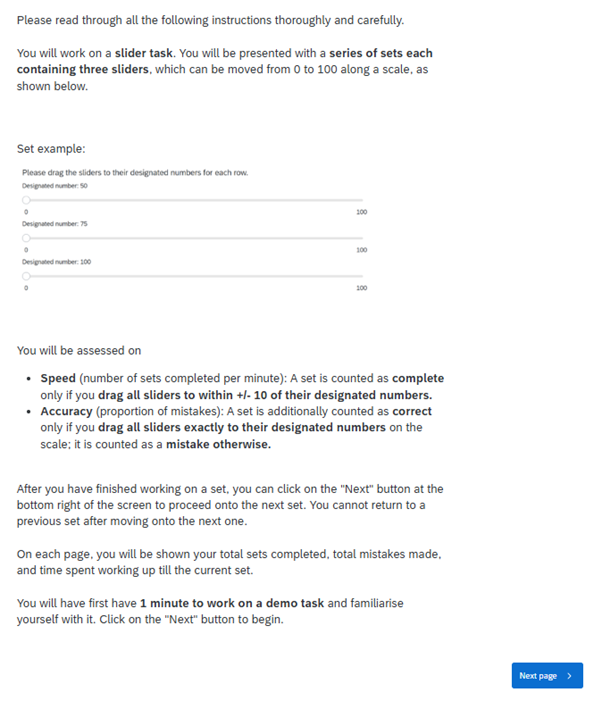
\includegraphics[width=\linewidth,height=0.9\textheight,keepaspectratio]{survey_screenshots/common_instructions.png}
\caption{Common instructions for all subjects}\label{fig-common-instructions}
\end{figure}

\begin{figure}[p]
\centering
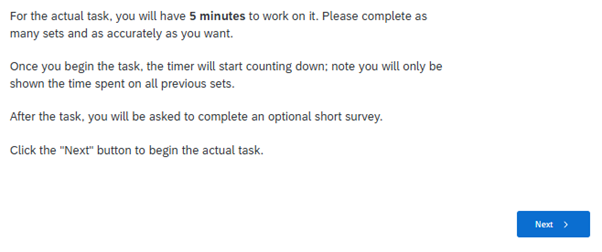
\includegraphics[width=\linewidth,height=0.9\textheight,keepaspectratio]{survey_screenshots/treatment1_instructions.png}
\caption{Treatment 1 instructions}\label{fig-treatment1-instructions}
\end{figure}

\begin{figure}[p]
\centering
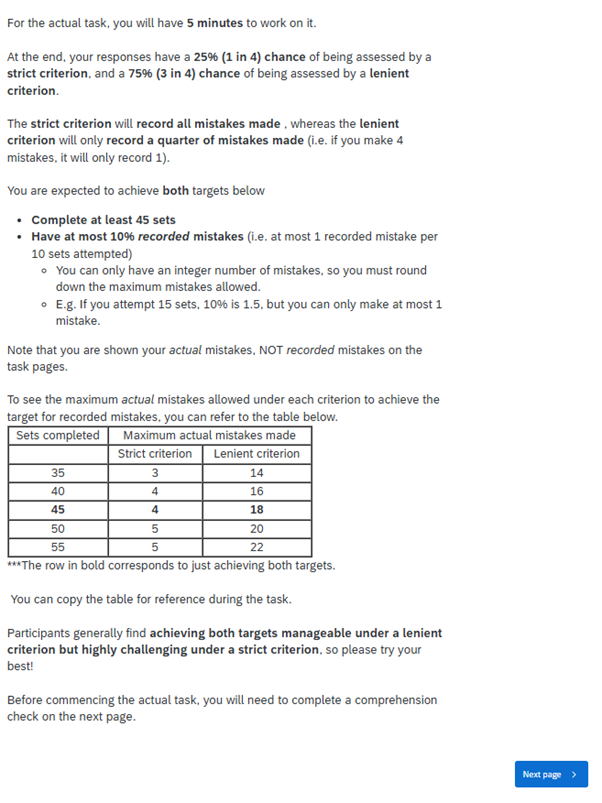
\includegraphics[width=\linewidth,height=0.9\textheight,keepaspectratio]{survey_screenshots/treatment2_instructions.png}
\caption{Treatment 2 instructions}\label{fig-treatment2-instructions}
\end{figure}

\begin{figure}[p]
\centering
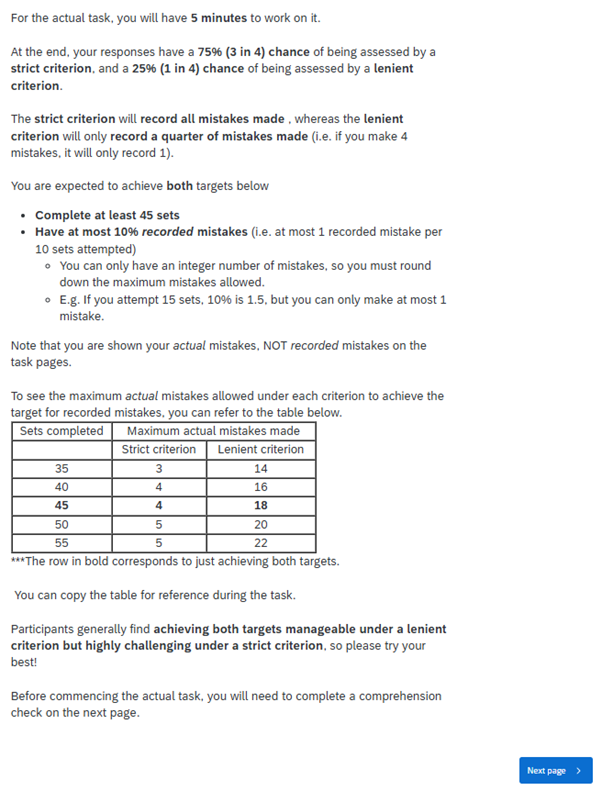
\includegraphics[width=\linewidth,height=0.9\textheight,keepaspectratio]{survey_screenshots/treatment3_instructions.png}
\caption{Treatment 3 instructions}\label{fig-treatment3-instructions}
\end{figure}

\begin{figure}[p]
\centering
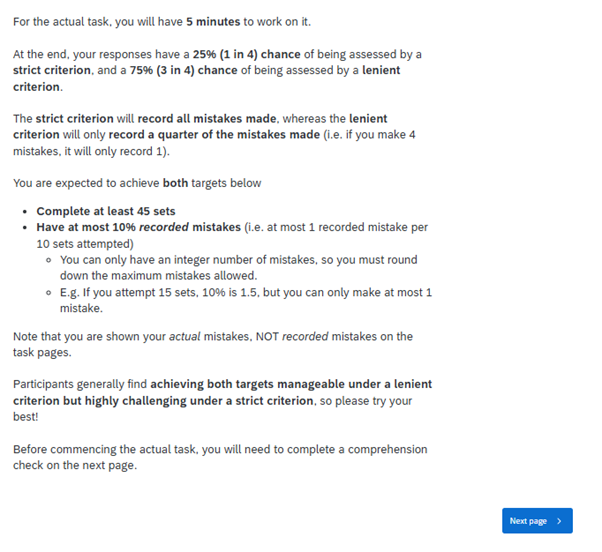
\includegraphics[width=\linewidth,height=0.9\textheight,keepaspectratio]{survey_screenshots/treatment4_instructions.png}
\caption{Treatment 4 instructions}\label{fig-treatment4-instructions}
\end{figure}

\begin{figure}[p]
\centering
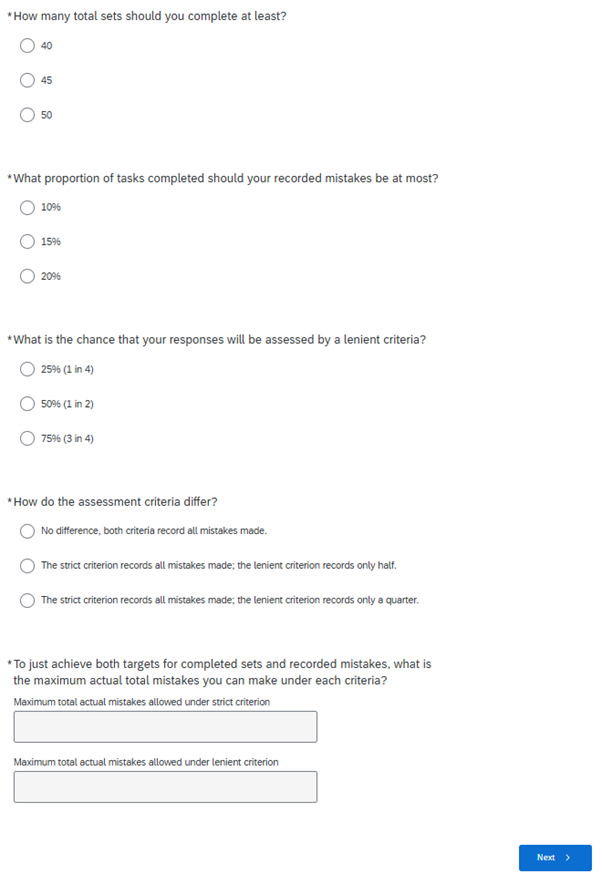
\includegraphics[width=\linewidth,height=0.9\textheight,keepaspectratio]{survey_screenshots/comprehension_check.png}
\caption{Comprehension check: last question only for treatments 2 and 3}\label{fig-compre-check}
\end{figure}

\begin{figure}[p]
\centering
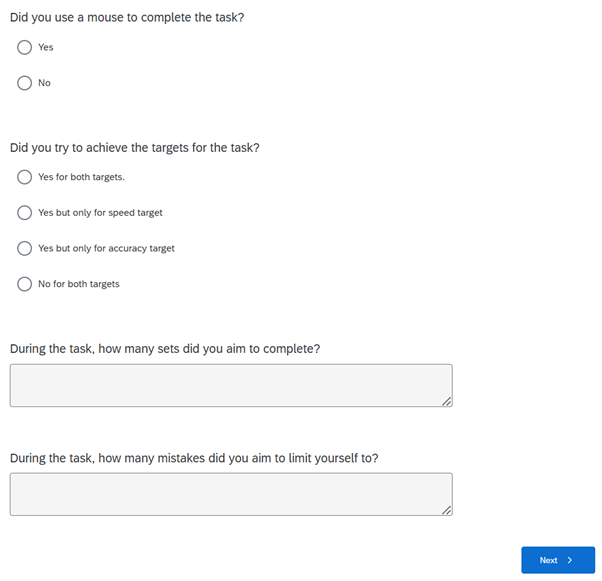
\includegraphics[width=\linewidth,height=0.9\textheight,keepaspectratio]{survey_screenshots/task_reflection_1.png}
\caption{Task reflection page 1}\label{fig-task-reflection-1}
\end{figure}

\begin{figure}[p]
\centering
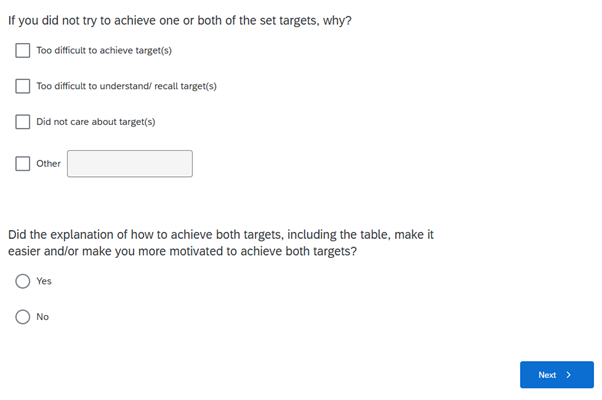
\includegraphics[width=\linewidth,height=0.9\textheight,keepaspectratio]{survey_screenshots/task_reflection_2.png}
\caption{Task reflection page 2}\label{fig-task-reflection-2}
\end{figure}

\begin{figure}[p]
\centering
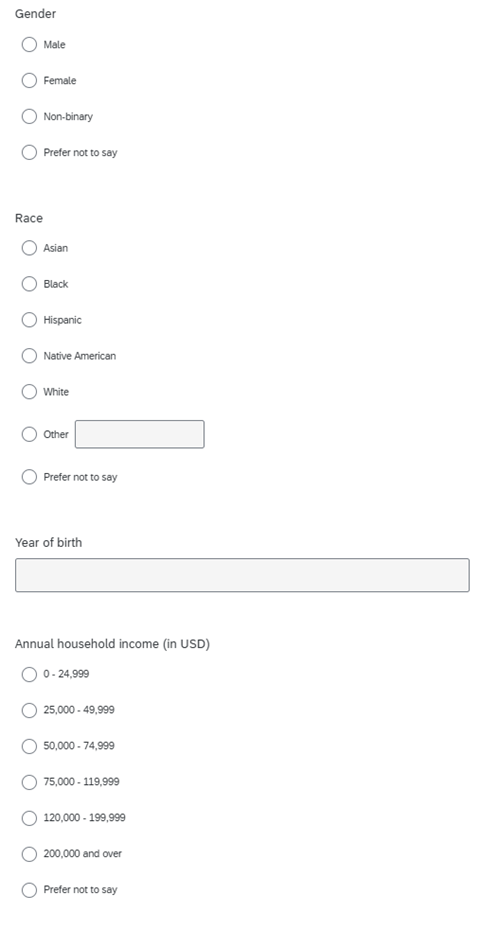
\includegraphics[width=\linewidth,height=0.9\textheight,keepaspectratio]{survey_screenshots/demographic_survey_1.png}
\caption{Demographic survey page 1}\label{fig-demographic-survey-1}
\end{figure}

\begin{figure}[p]
\centering

\includegraphics[width=\linewidth,height=0.9\textheight,keepaspectratio]{survey_screenshots/demographic_survey_2.png}
\caption{Demographic survey page 2}\label{fig-demographic-survey-2}
\end{figure}

\begin{figure}[p]
\centering
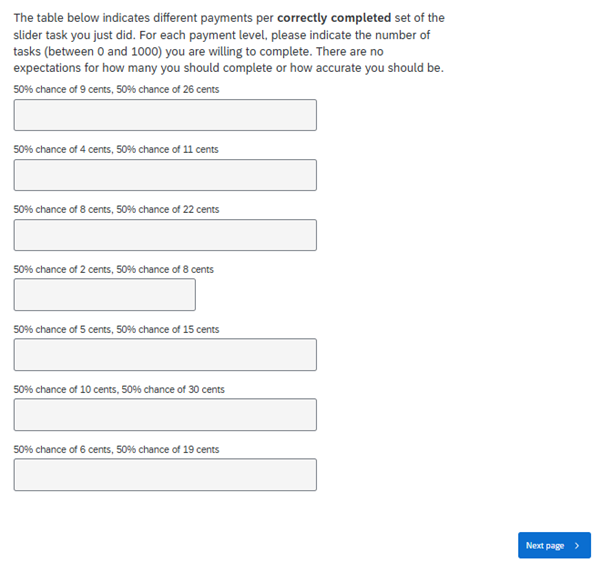
\includegraphics[width=\linewidth,height=0.9\textheight,keepaspectratio]{survey_screenshots/loss_aversion_survey_1.png}
\caption{Loss aversion survey page 1: pages and payment structures presented in random order}\label{fig-loss-aversion-survey-1}
\end{figure}

\begin{figure}[p]
\centering
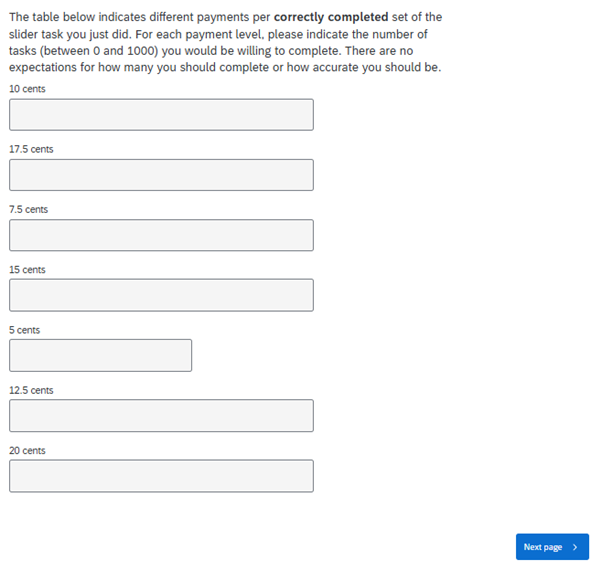
\includegraphics[width=\linewidth,height=0.9\textheight,keepaspectratio]{survey_screenshots/loss_aversion_survey_2.png}
\caption{Loss aversion survey page 2: pages and payment structures presented in random order}\label{fig-loss-aversion-survey-2}
\end{figure}

\end{document}
